%\section{Tutkimusaineisto ja -menetelmät}
\section{Design process \& methods}
\label{sec:ojectives}

\subsection{Design objectives}
The objective of this thesis is to study feasible antenna structures for metal-covered mobile phones. The phone should have two similar cellular antennas (main and diversity) for MIMO operation. Additionally, two antennas to operate on GPS and Wi-Fi frequencies are to be designed. To clarify, from now on, main antenna refers to the first cellular antenna to be designed, and diversity antenna to the second one, regardless how their final performances will compare to each other. Table \ref{tab:design_goals} below presents the goals and requirements for this project.

\begin{table}[H]
    \centering
    \caption{Criteria for the antennas to be designed.}
    \label{tab:design_goals}
    \begin{tabular}{|l|c|}
        \hline
         \textbf{Parameter} & \textbf{Value} \\
         \hline
         Reflection coefficient & $S_{11} < -5\,\db$\\
         \hline
         Cellular efficiency & $\eta > 30\,\%$\\
         \hline
         Isolation between main and diversity antenna & $S_{21} < -15\,\db$\\
         \hline
         GPS/Wi-Fi efficiency & $\eta > 40\,\%$\\
         \hline\hline
         \textbf{Frequencies} & \\
         \hline
         Main cellular antenna & $0.704-0.960\,\giga\hertz, 1.71-2.69\,\giga\hertz$\\
         \hline
         Diversity cellular antenna & $0.704-0.960\,\giga\hertz, 1.71-2.69\,\giga\hertz$\\
         \hline
         GPS antenna & $1.56-1.61\,\giga\hertz$\\
         \hline
         Wi-Fi antenna & $2.4-2.484\,\giga\hertz, 5.15-5.875\,\giga\hertz$\\
         \hline
    \end{tabular}
\end{table}


\subsection{Design strategy}
\label{sec:process}
Electromagnetic (EM) simulations were made in CST Microwave Studio \cite{cst}. It was used to create antenna and phone models, and to calculate system's $S$-parameters. Simulations were focused on antenna's initial matching, i.e. $S_{11}$ for each antenna. The procedure of testing different antenna structures was pretty straightforward: first a model was built, then simulated, and finally the obtained results were analyzed. Based on the previous findings, the model was modified aiming to wide impedance matching, and then simulated again. The first tests were done with a simple model and a simple antenna design. While the antenna structures got better, the model of the phone was also modified to be more realistic.

Antennas were designed in order of significance. The cellular antennas were considered more important, and thus they were studied first. Development process of the antennas began with the main antenna, and when it was operating properly, the same process was applied to design the diversity antenna. The final step was to add solutions for GPS and Wi-Fi antennas. Figure \ref{fig:ant_order} illustrates the proceeding order. 

The basic research strategy was first to find solution for the main antenna to operate on the lower frequency band (LB, $704-960\,\mega\hertz$). Lower band was designed first, since it is harder to reach the determined matching levels and efficiencies at lower frequencies. Results from the previous studies have shown weaker performance at those areas. Also, the required antenna structures might be larger, which makes them more critical to be prioritized due to the already limited available space. After a reasonable performance was achieved at that band, the model was configured to support also the higher frequency band (HB, $1.71-2.69\,\giga\hertz$). Accordingly, the design of GPS/Wi-Fi antennas was started from the lowest frequency, i.e. GPS ($1.56-1.61\,\giga\hertz$), after which, the Wi-Fi frequencies ($2.4-2.484\,\giga\hertz$ and $5.15-5.875\,\giga\hertz$) were added. The process flow of designing one antenna is visualized in Figure \ref{fig:ant_design}.

Before moving on the next antenna, the design constraints had to be checked. One antenna was iterated until the targets were reached (Figure \ref{fig:step}). When the antenna under development was performing according to the requirements, or at least at a decent level, the design of a another antenna was started.

Designing antennas was not limited only in antenna structures. In order to reach the goals presented above, matching networks were to be designed as well. Finding usable circuit topologies was done simultaneously with EM simulations. Optenni Lab \cite{optenni} and NI AWR Design Environment \cite{awr} were used for this purpose. The $S$-parameter file obtained from CST-simulations was given to and read by these programs. Optenni searches for the best matching circuit according to given frequency band settings and amount of circuit elements. Resulted circuits were modified and fine-tuned in AWR, to reach the defined design objectives. Also, in AWR the ideal circuit elements were later replaced with Spice-models of actual components to obtain more realistic results.

\begin{figure}[H]
    \centering
    \begin{subfigure}[b]{\textwidth}
        \begin{tikzpicture}[node distance=2cm]
            \node (main) [antenna] {Main antenna};
            \node (div) [antenna, right of=main, xshift=2cm] {Diversity antenna};
            \node (gps1) [antenna, right of=div, xshift=2cm] {GPS/Wi-Fi antenna 1};
            \node (gps2) [antenna, right of=gps1, xshift=2cm] {GPS/Wi-Fi antenna 2};
            \draw [arrow] (main) -- (div);
            \draw [arrow] (div) -- (gps1);
            \draw [arrow] (gps1) -- (gps2);
        \end{tikzpicture}
        \caption{Design order of the required antennas.}
        \label{fig:ant_order}
    \end{subfigure}
    
    \begin{subfigure}[b]{\textwidth}
        \begin{tikzpicture}[node distance=2cm]
            \node (ant) [antenna] {New antenna};
            \node (que) [query, right of=ant, xshift=2cm] {Antenna type};
            \node (lb) [block, right of=que, xshift=0.5cm, yshift=-1.5cm] {LB};
            \node (hb) [block, right of=lb, xshift=0.5cm] {HB};
            \node (mc) [block, right of=hb, xshift=0.5cm] {MC};
            \node (gps) [block, right of=que, xshift=0.5cm, yshift=1.5cm] {GPS};
            \node (wifi24) [block, right of=gps, xshift=0.5cm] {2.4\,GHz};
            \node (wifi5) [block, right of=wifi24, xshift=0.5cm] {5\,GHz};
            \draw [arrow] (ant) -- (que);
            \draw [arrow] (que) |- node[anchor=north] {cellular} (lb);
            \draw [arrow] (lb) -- (hb);
            \draw [arrow] (hb) -- (mc);
            \draw [arrow] (que) |- node[anchor=south] {GPS/Wi-Fi} (gps);
            \draw [arrow] (gps) -- (wifi24);
            \draw [arrow] (wifi24) -- (wifi5);
            \draw [arrow] (wifi5) -- (mc);
            \draw [arrow] (mc) -- +(0,-1) -| (ant);
        \end{tikzpicture}
        \caption{Design process of an antenna.}
        \label{fig:ant_design}
    \end{subfigure}
\end{figure}  

\begin{figure}[H]
    \centering
    \ContinuedFloat
    \begin{subfigure}[b]{\textwidth}
        \begin{tikzpicture}[node distance=2cm]
            \node (ant) [antenna] {Antenna to design};
            \node (que) [query, right of=ant, xshift=2cm] {Targets reached?};
            \node (ant2) [antenna, right of=que, xshift=3cm] {Next antenna};
            \draw [arrow] (ant) -- (que);
            \draw [arrow] (que) -- node[anchor=south] {yes} (ant2);
            \draw [arrow] (que) -- +(0,-2.5)-| (ant)  node[near start,sloped,below] {no} ;
        \end{tikzpicture}
        \caption{A single step of the whole process.}
        \label{fig:step}
    \end{subfigure}
    \caption{Flowcharts illustrating the design procedure.}
    \label{fig:flowcharts}
\end{figure}


\subsection{Electromagnetic model of the mobile phone}
\label{sec:phone}
Besides the antennas, also the phone had to be modeled electromagnetically. For this project it was specified to use a mechanically accurate model, shown in Figure \ref{fig:cad}. However, this model is too detailed for research purposes, and thus it will be modified, which is explained more in section \ref{sec:sim_realistic}. The model anyway consists of metallic back cover and side frame, plastic structure, and some subsystems of a phone. Metallic parts, and all of the subsystems and other parts were modeled as perfect electric conductors (PEC) to reduce simulation times. The plastic rim was the only non-metallic part of the model.
\begin{figure}[H]
    \centering
    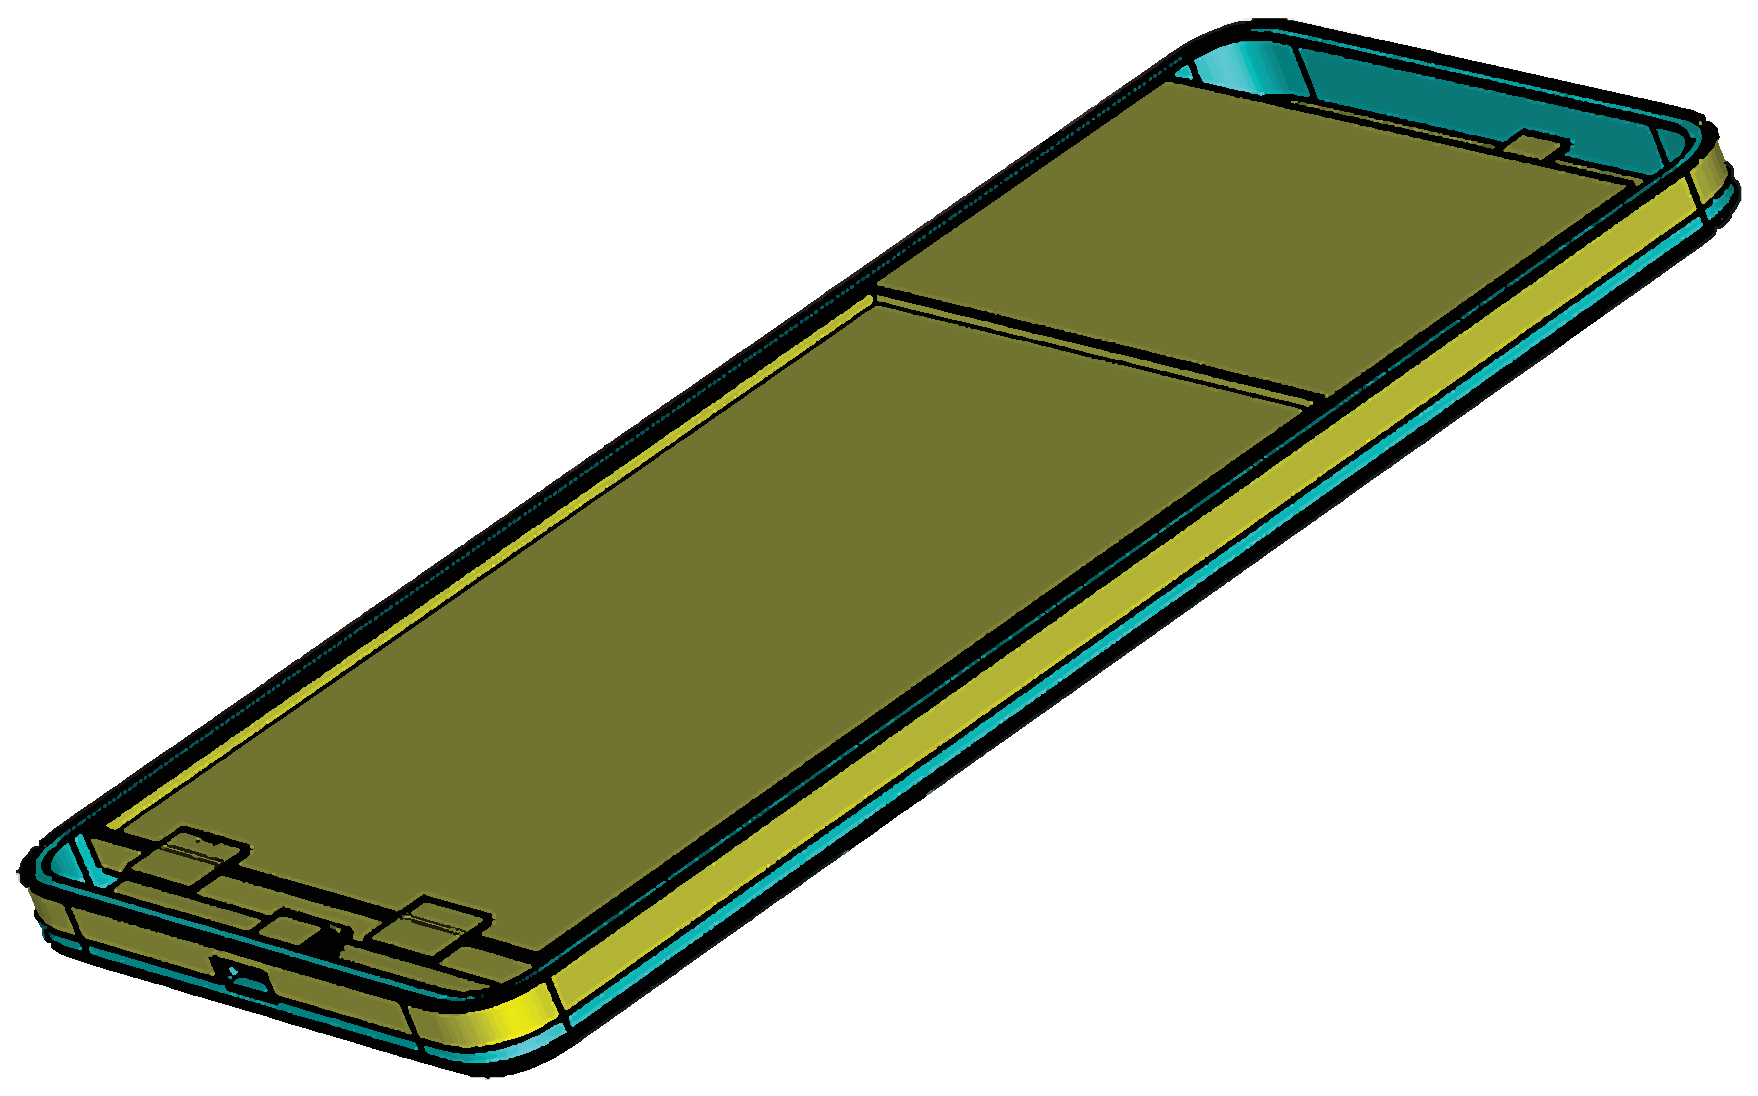
\includegraphics[width=0.6\textwidth]{img/cad.eps}
    \caption{3D-model of a smart phone.}
    \label{fig:cad}
\end{figure}

Before the precise model was taken into use, simulations were first done with a plain model. Basically, that was a PEC-sheet for back cover, and a FR4-substrate with a another PEC-sheet to model the display. Figure \ref{fig:basic_structure} illustrates that model, and has also the key dimensions of the phone marked into it. The antennas were built to the empty sides of the model, and eventually they would be integrated to the side frame of the accurate model. The simple model was used until a promising structure for the main antenna was found. 
\begin{figure}[H]
    \centering
    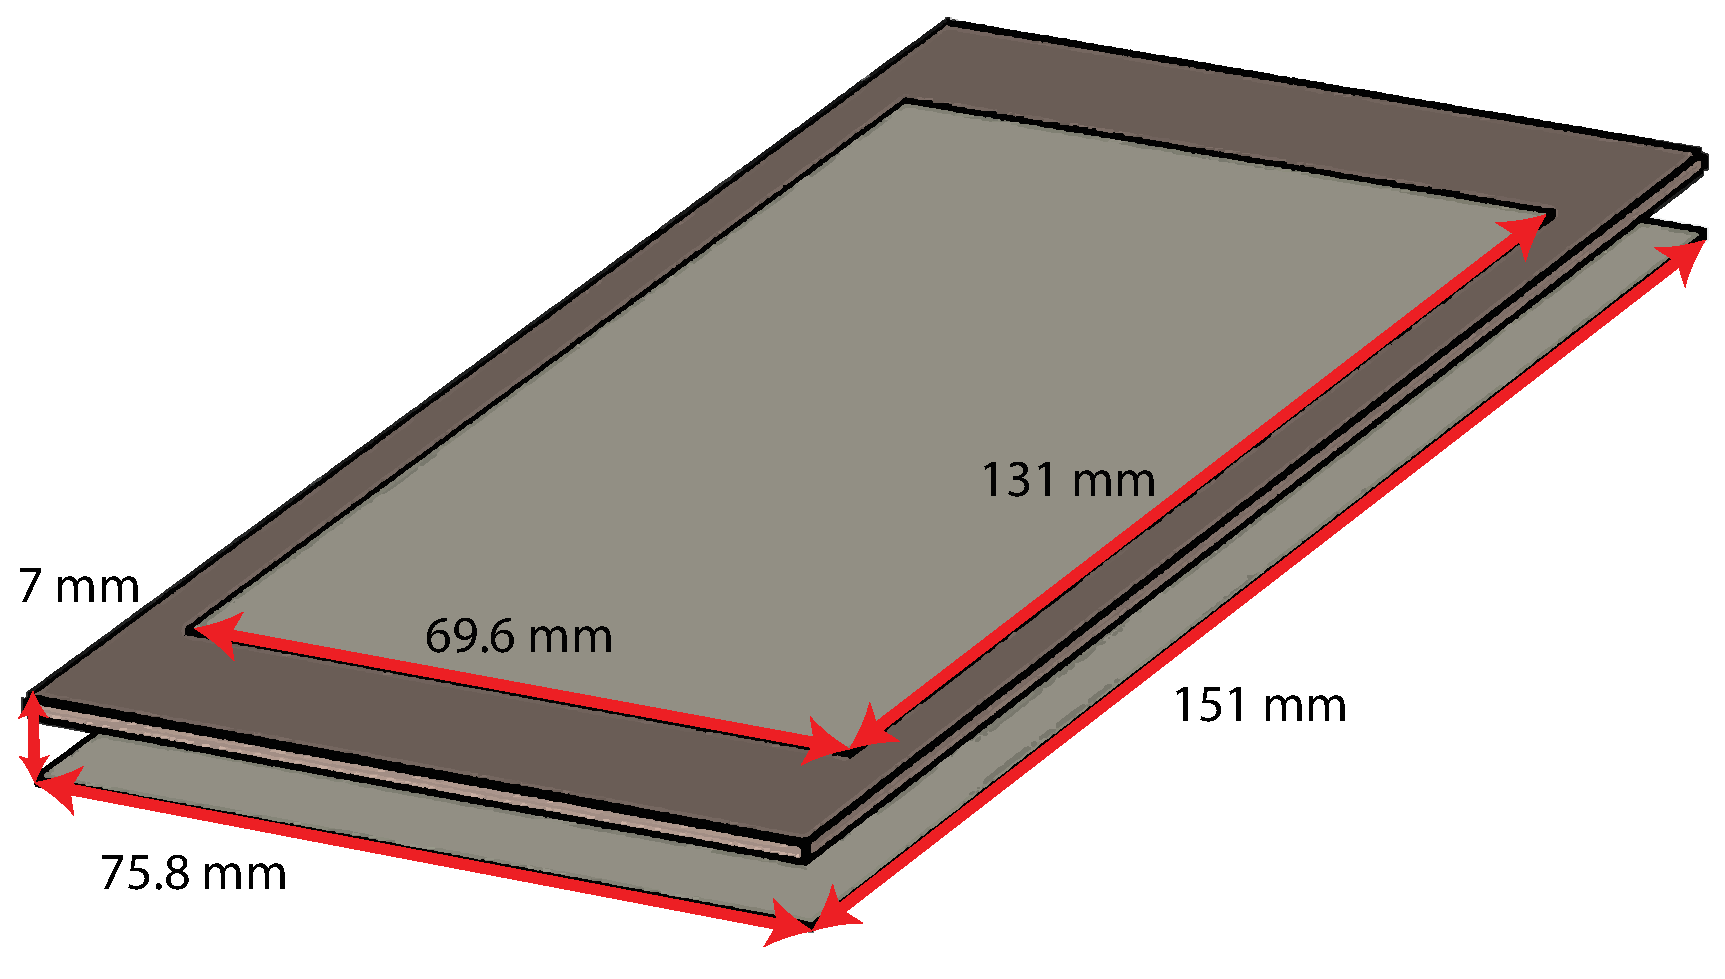
\includegraphics[width=0.6\textwidth]{img/basic_structure.eps}
    \caption{Simplified, basic model of a mobile phone to be used in simulations.}
    \label{fig:basic_structure}
\end{figure}

\subsection{Preliminary antenna study}
\label{sec:pre_study}
The first simulations with the plain model were about gathering knowledge on how different structures perform in the presence of the metal cover. Gaining this information was critical since antennas in metal-covered mobile phones are not that much studied, as was presented in section \ref{sec:full_cover}. This preliminary study (later also pre-study) focuses on different dimensions of antennas, their locations, shapes, feed positions, and the metal cover itself. The structures of antenna elements were kept as simple as possible in order to follow the effects of each parameter in an efficient way. 


\subsubsection{Effect of metal cover}
\label{sec:metal_effect}
The main point of interest, as well as the main challenge, is the metal cover and how it affects the antenna's performance. To demonstrate the complexity of this design project, simulations to test the effect of the metal were run. Since this test was just an example, simulation model was kept simple. A long, L-shaped antenna completely covering one long side and one short side, with a little square on the corner was used in this test. Models are shown in Figure \ref{fig:metal_vs_nometal_model}.

\begin{figure}[H]
    \centering
    \begin{subfigure}[b]{0.49\textwidth}
    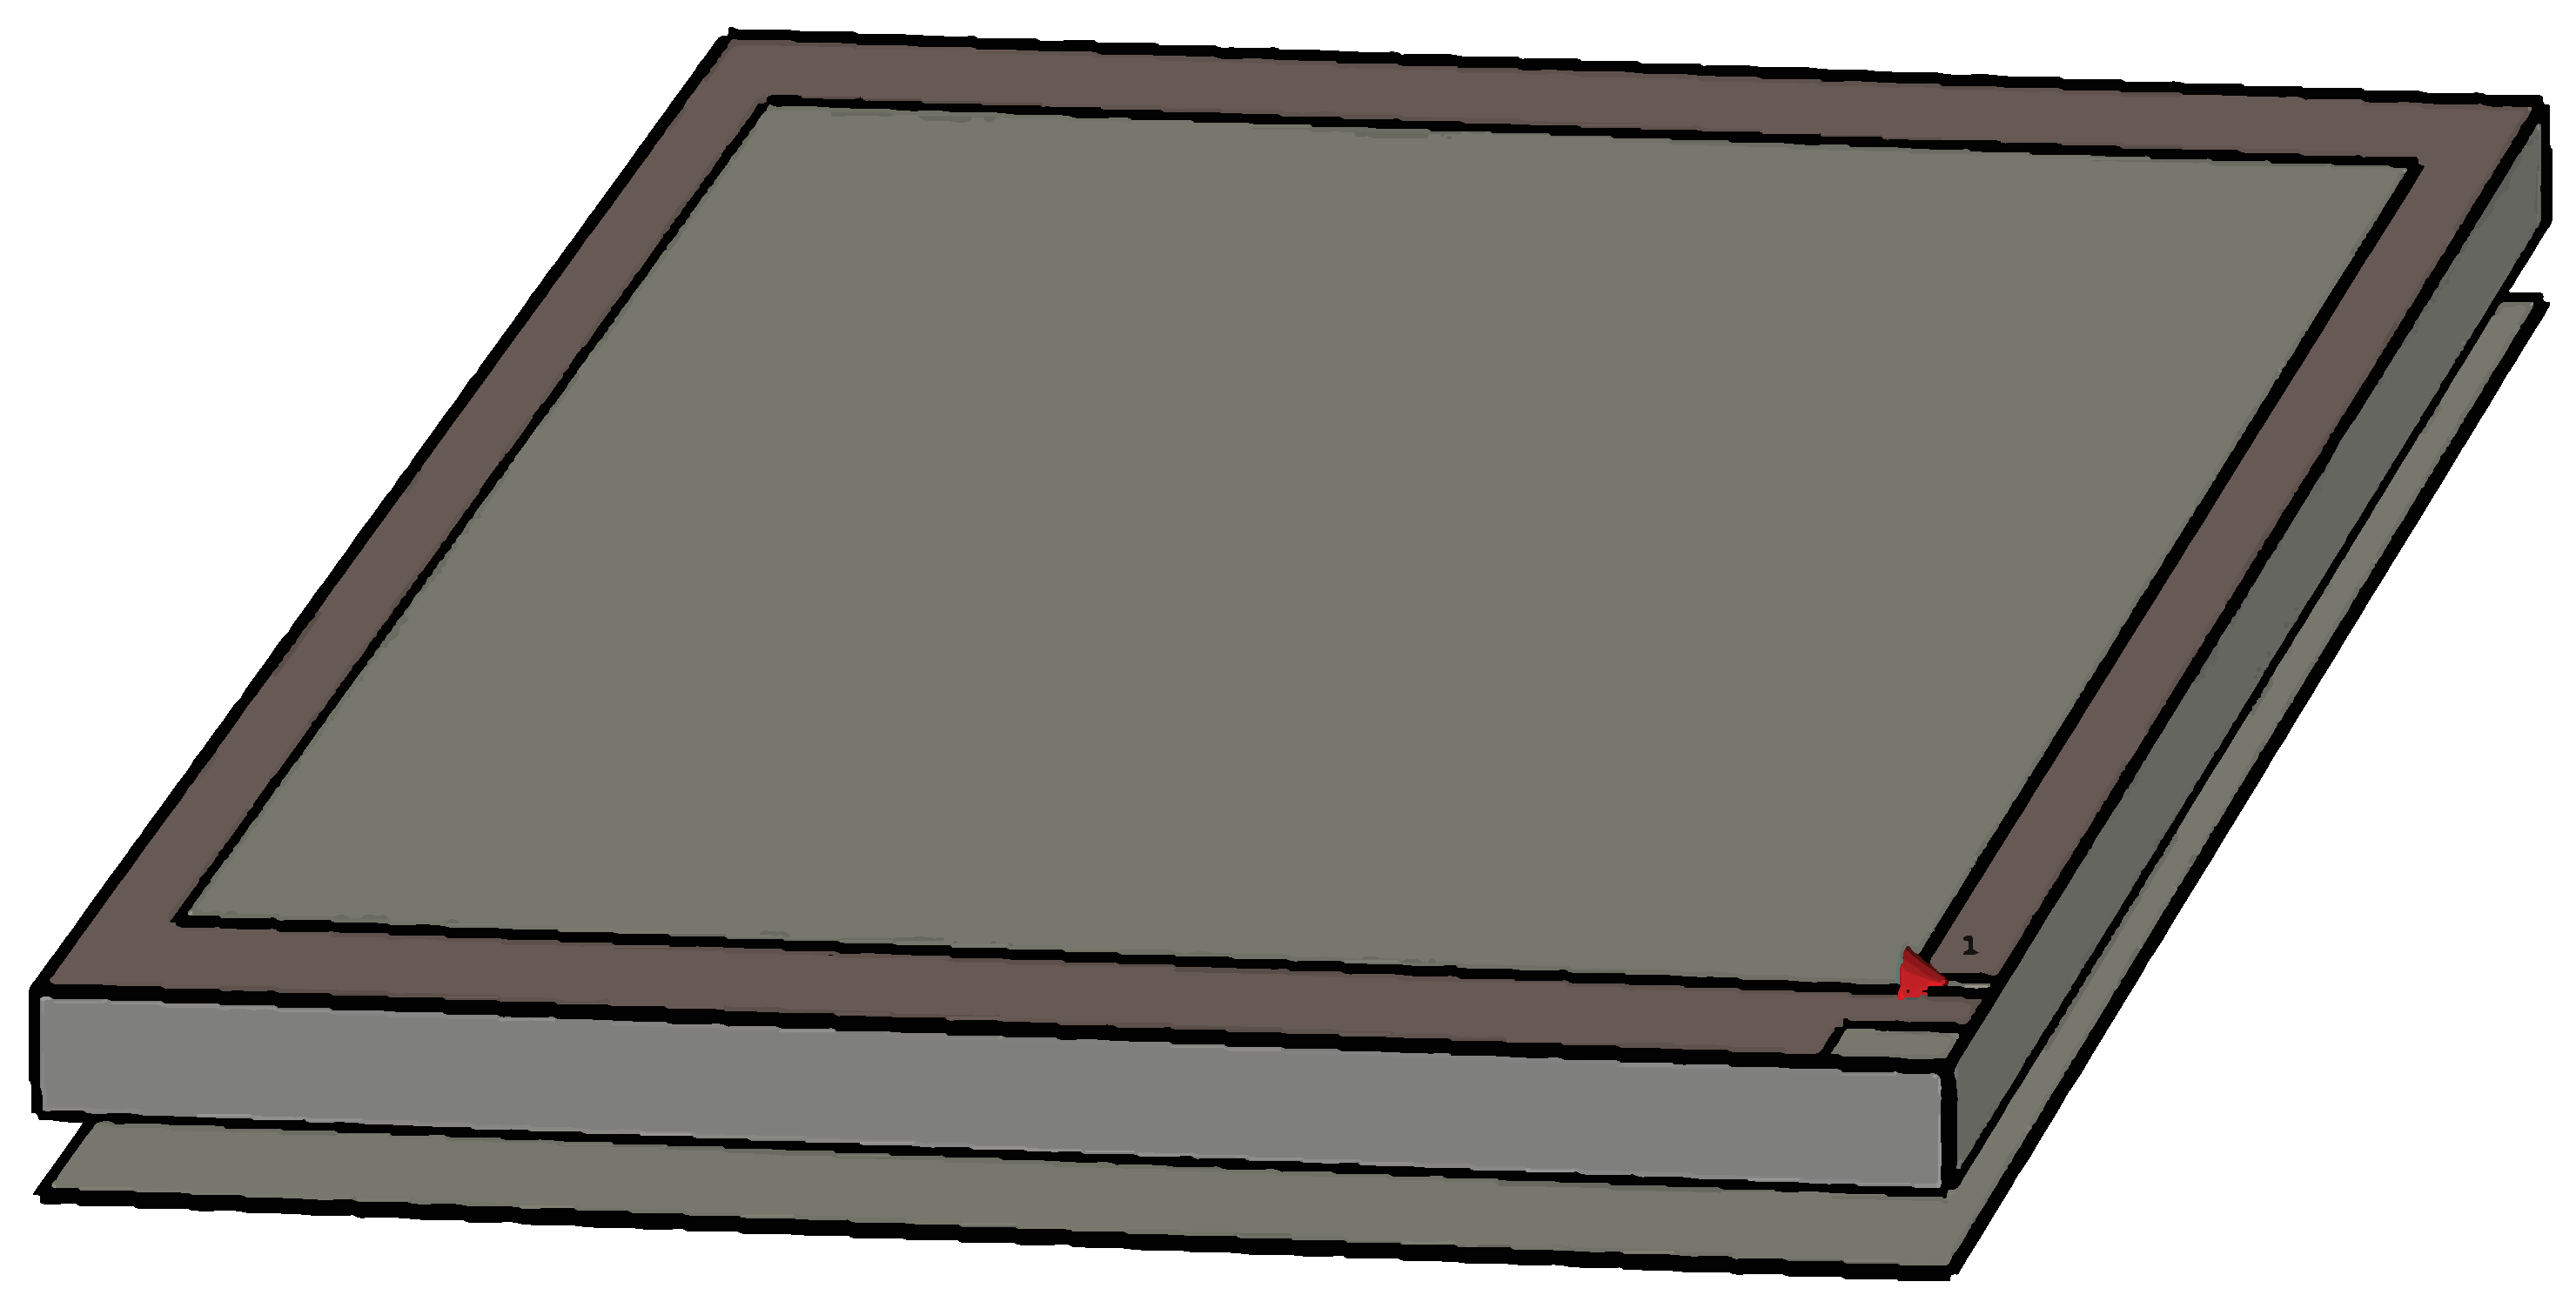
\includegraphics[width=\textwidth]{img/metal_cover.eps}
    \caption{With metal cover.}
    \label{fig:metal_cover}
    \end{subfigure}
    \begin{subfigure}[b]{0.49\textwidth}
    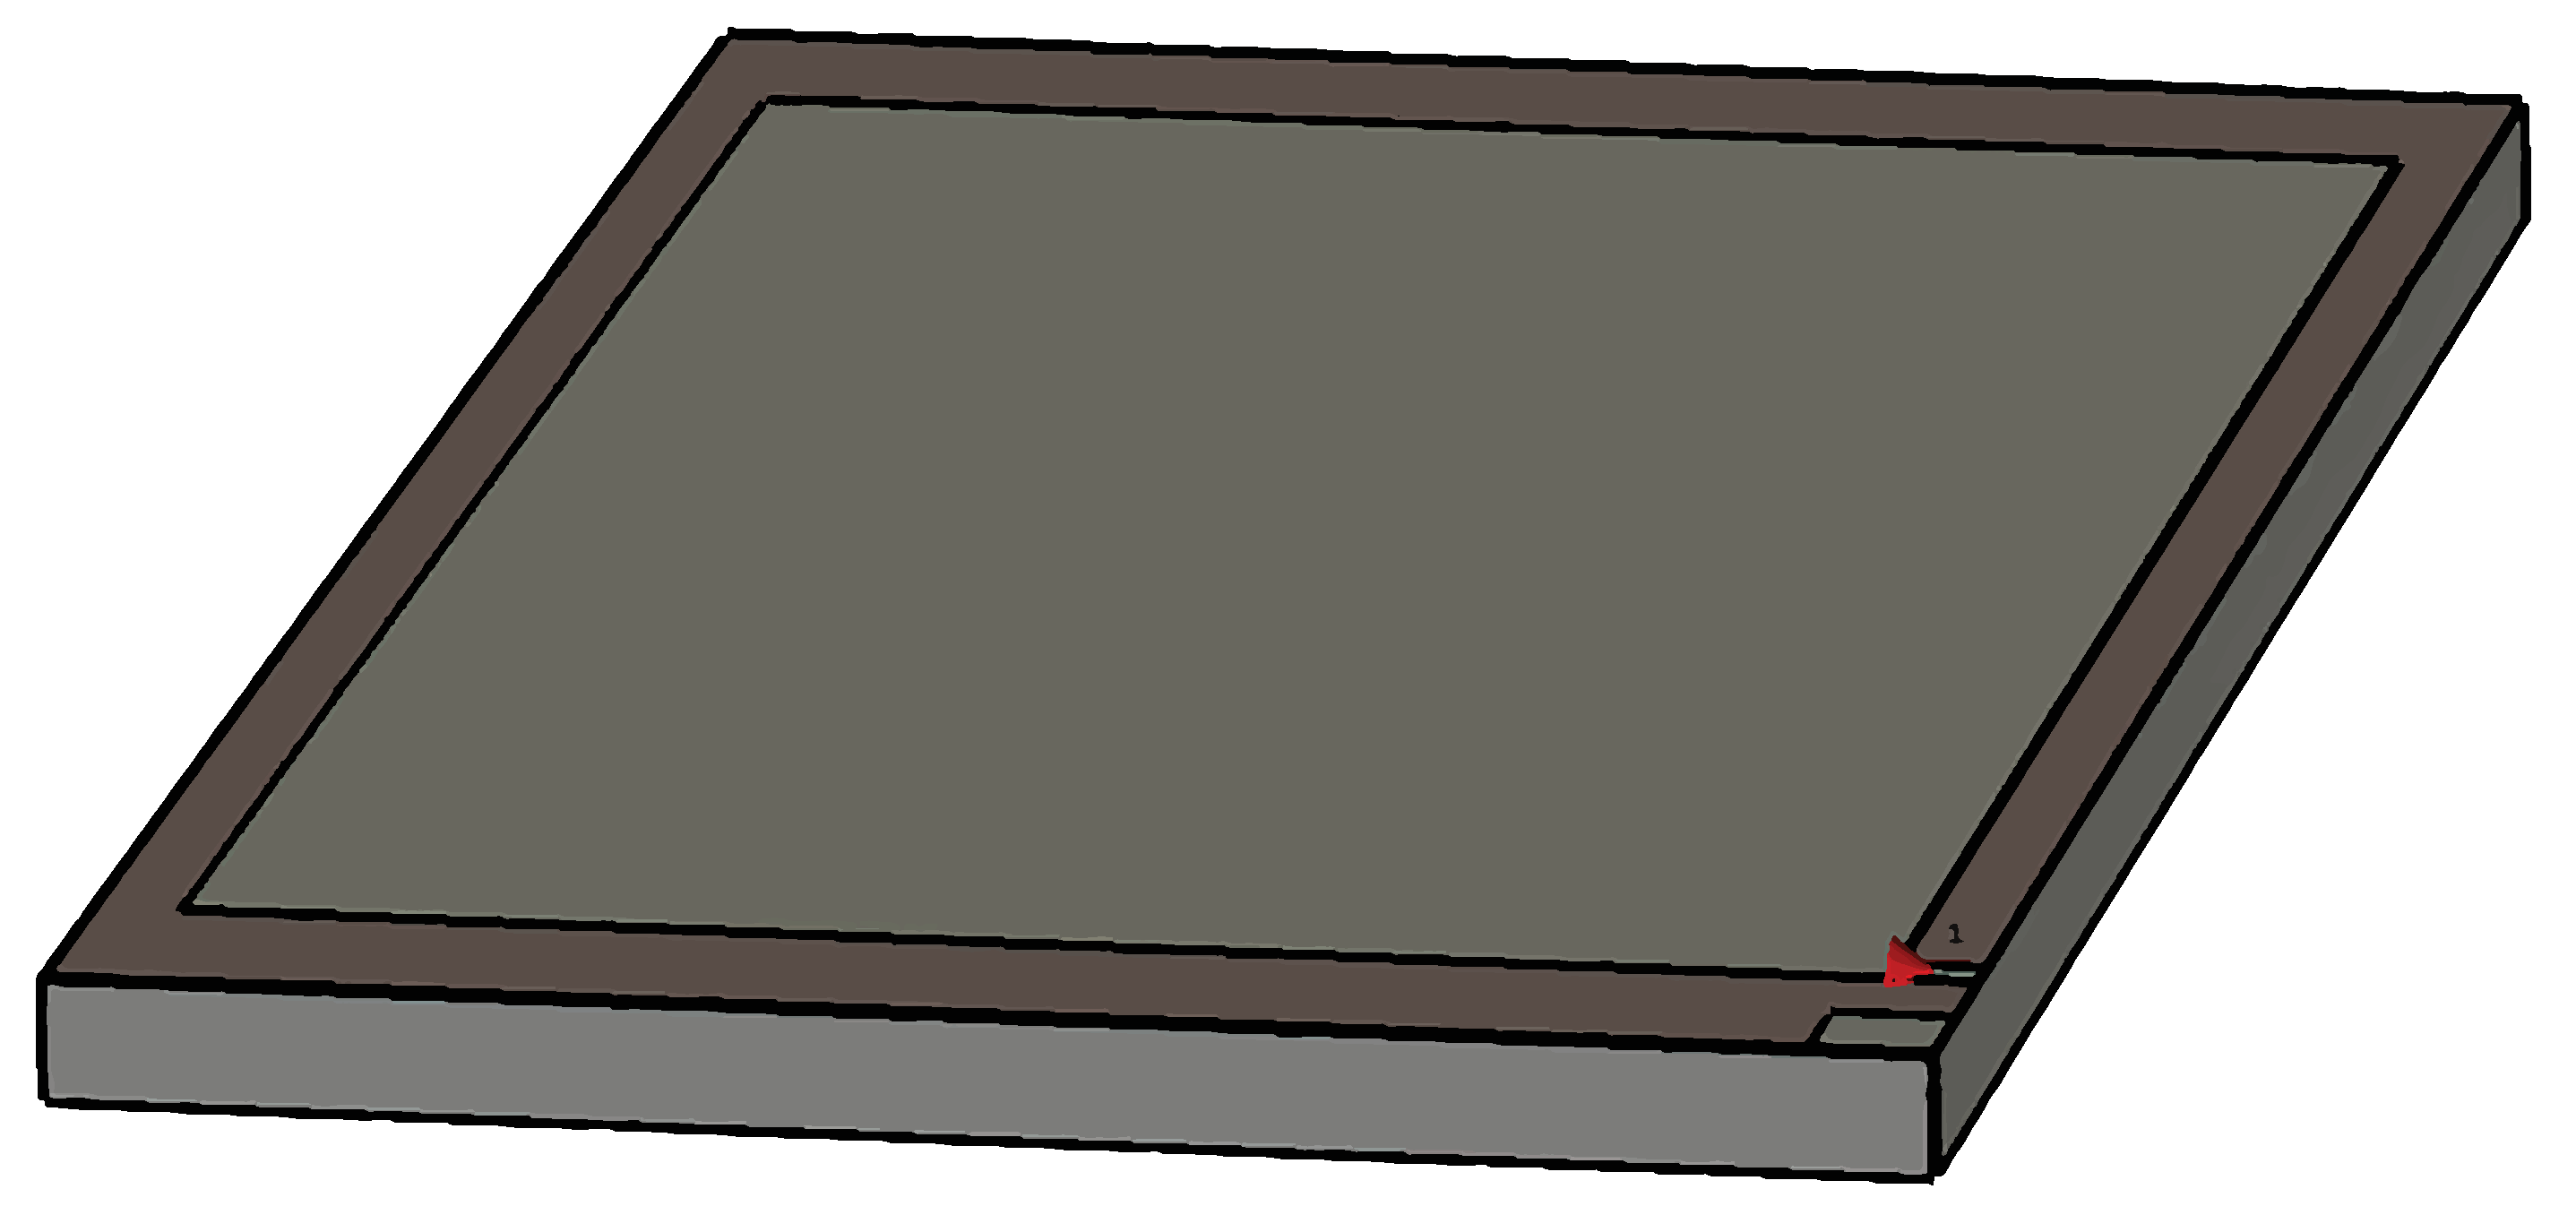
\includegraphics[width=\textwidth]{img/no_metal_cover.eps}
    \caption{Without metal cover.}
    \label{fig:nometal_cover}
    \end{subfigure}
    \caption{Simulation models used to test the effect of metal cover. Antenna element is on the side of the phone.}
    \label{fig:metal_vs_nometal_model}
\end{figure}

Figure \ref{fig:metal_vs_nometal} shows the results from the CST-simulation. The effect of the metal cover can be seen clearly. The blue curve has a metallic back cover while the red, dashed one does not. Looking at the low band reveals a major difference. The aim of the matching level is $-5\,\db$ and that is almost achieved when the metal cover is taken away without any external matching networks. With metal cover the antenna resonates more with narrower peaks and has no desired matching level at any frequency. 

Figure \ref{fig:metal_vs_nometal_matched} presents the same simulations with 4-element matching circuit created with Optenni Lab. This time the difference is even larger. Without metal cover the desired matching level is exceeded by far. In contrary, adding matching circuit to the other case is not much of help. Even though the level is now more constant in the band, it is far from acceptable.

\begin{figure}[H]
    \centering 
    \begin{subfigure}[b]{0.49\textwidth}
        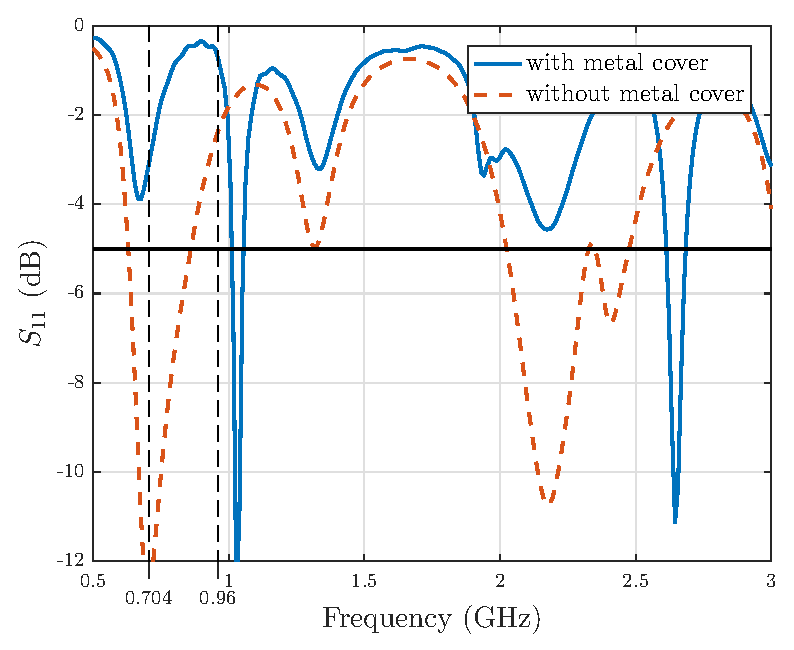
\includegraphics[width=\textwidth]{img/metal_vs_nometal.eps}
        \caption{Without matching circuit.}
        \label{fig:metal_vs_nometal}
    \end{subfigure}
    \begin{subfigure}[b]{0.49\textwidth}
        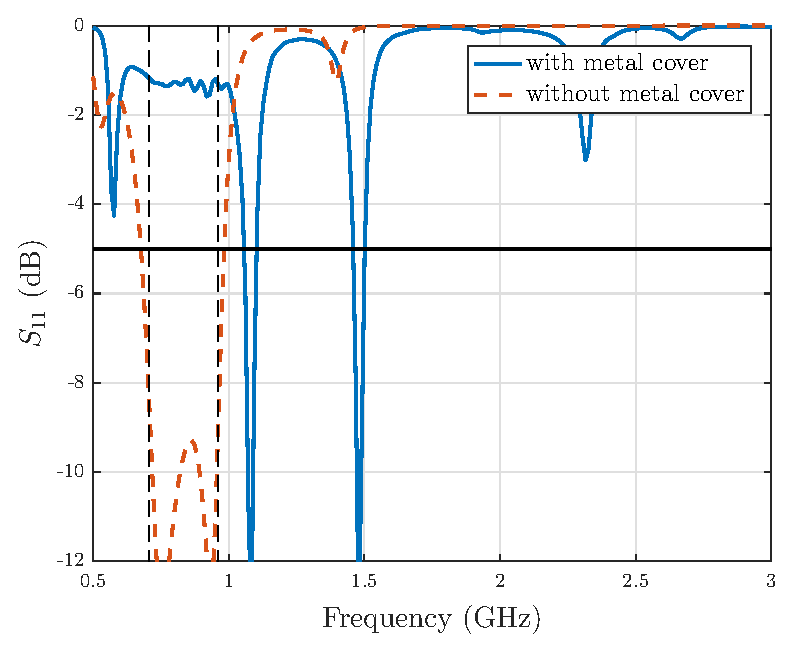
\includegraphics[width=\textwidth]{img/metal_vs_nometal_matched.eps}
        \caption{Matched antennas.}
        \label{fig:metal_vs_nometal_matched}
    \end{subfigure}
    \caption{Effect of the metal back cover on antenna performance.}
    \label{fig:metal_vs_nometal_results}
\end{figure}



\subsubsection{Size of an antenna}
\label{sec:antenna_size}
As mentioned earlier in section \ref{sec:process}, antennas were designed and developed in the EM simulator. Each simulated design provided information that was useful for the following iterations. 

The first interesting metric to investigate was the size of the antenna. This meant length ($l$) and width ($w$) of the antenna since all elements were considered as thin metallic sheets. The tested antennas were $2\,\milli\meter$ wide metal strips either on the long or the short side of the phone (see Figures \ref{fig:ant_length_long} and \ref{fig:ant_length_short}, respectively). In both cases everything else was kept constant except the length of antenna. 

\begin{figure}[H]
    \centering
    \begin{subfigure}[b]{0.49\textwidth}
        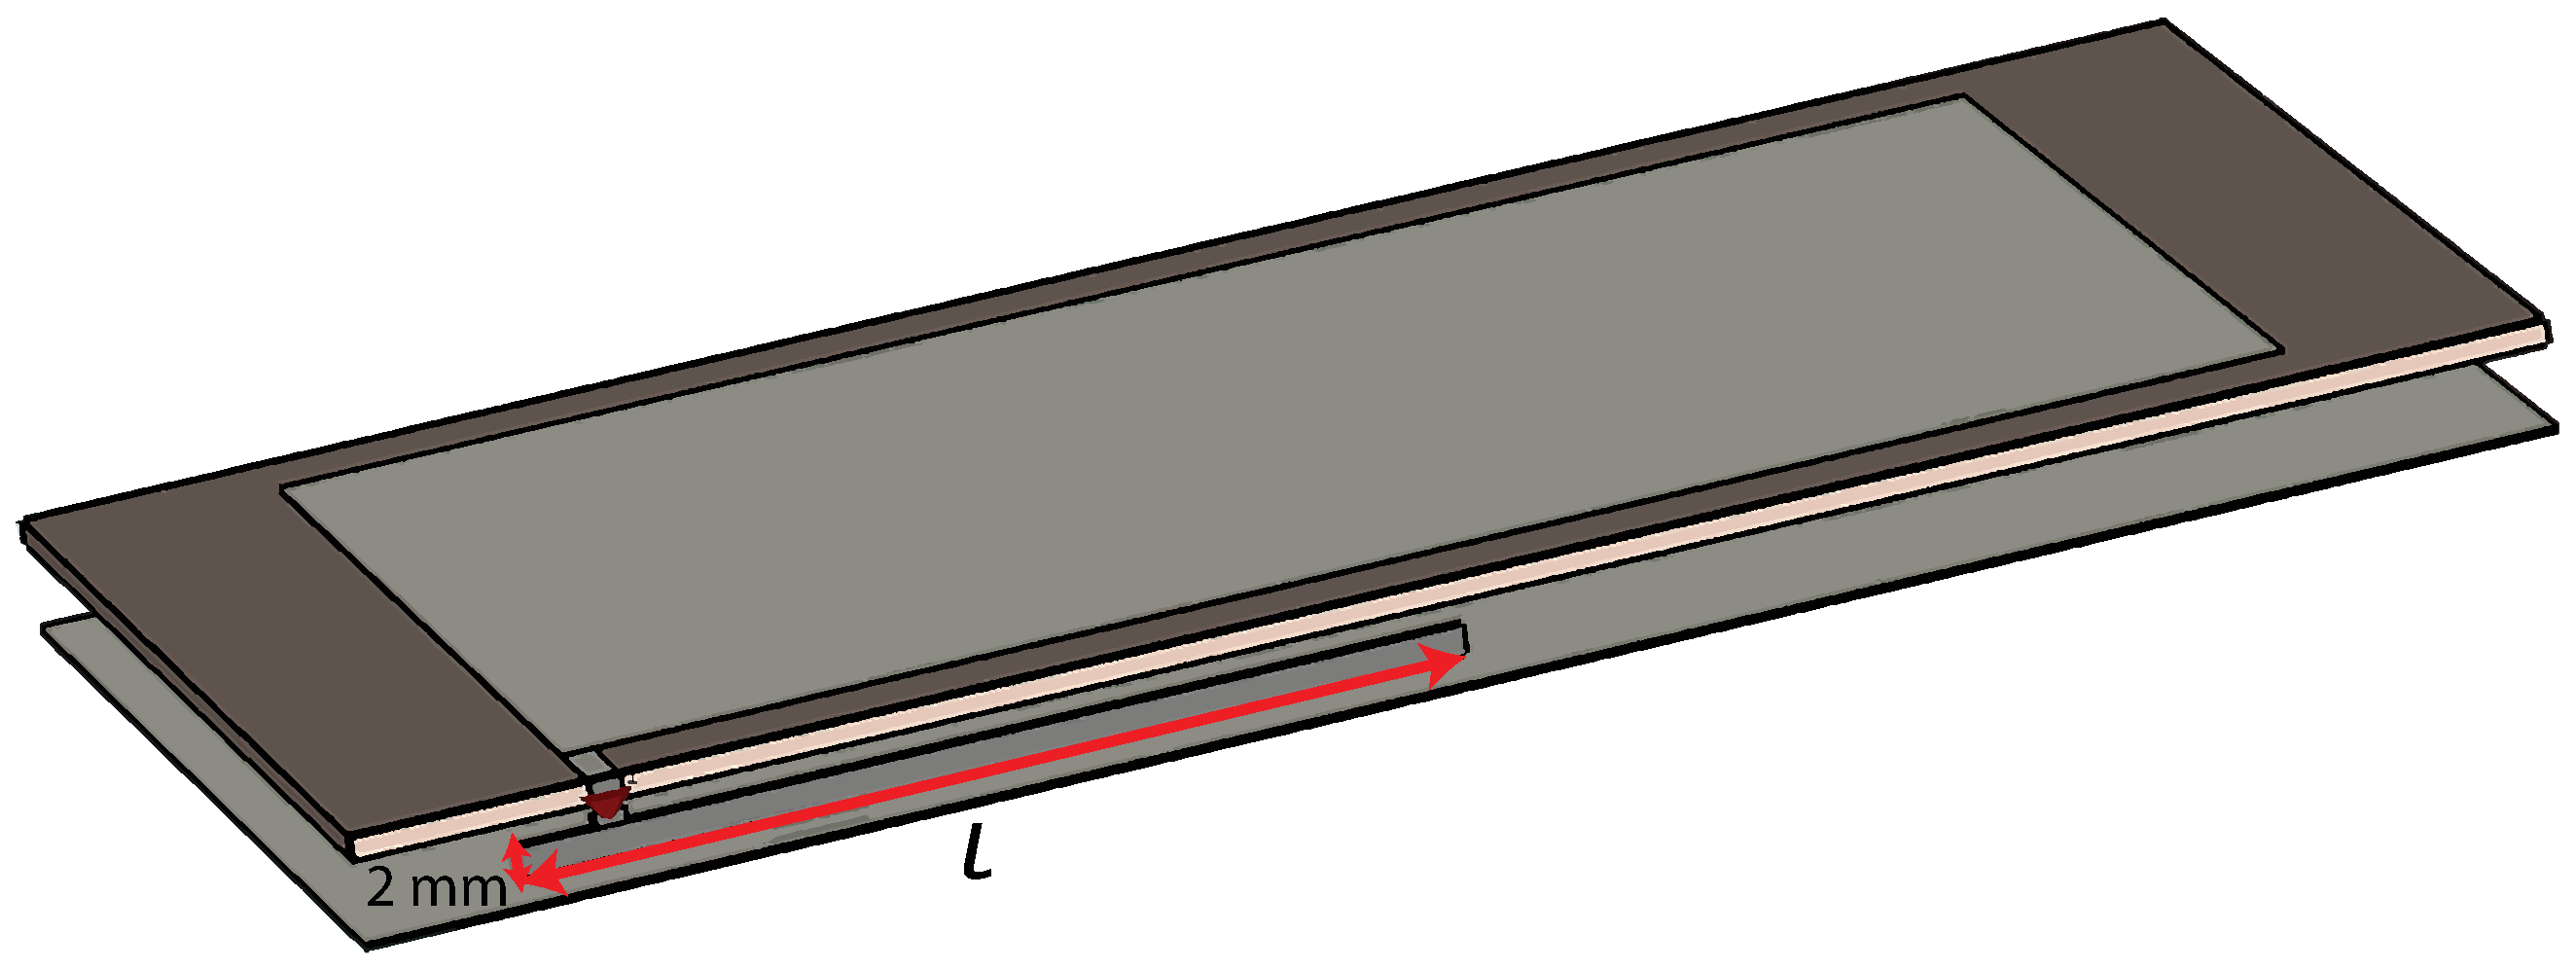
\includegraphics[width=\textwidth]{img/ant_length_long.eps}
        \caption{Antenna located on the side of the phone.}
        \label{fig:ant_length_long}
    \end{subfigure}
    \begin{subfigure}[b]{0.49\textwidth}
        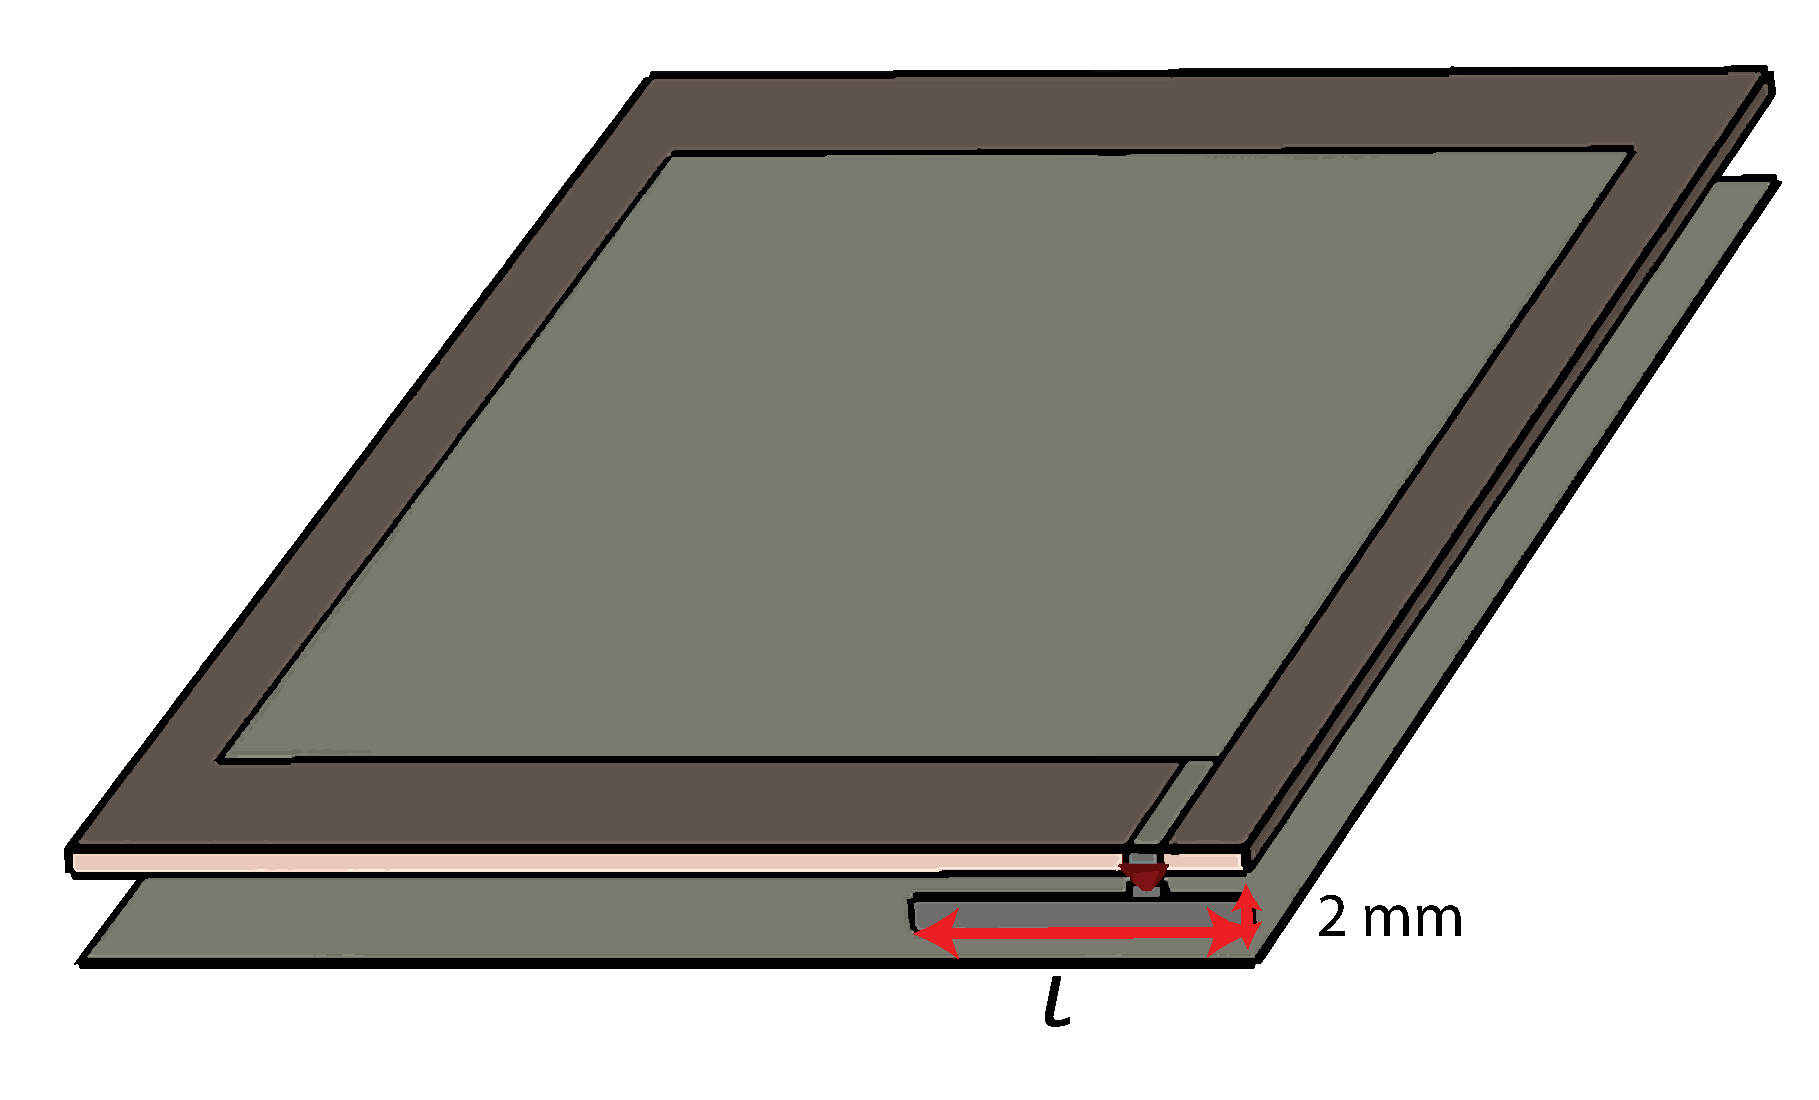
\includegraphics[width=\textwidth]{img/ant_length_short.eps}
        \caption{Antenna located on the top of the phone.}
        \label{fig:ant_length_short}
    \end{subfigure}
    \caption{Models used to test the effect of antenna's length.}
    \label{fig:ant_length_model}
\end{figure}

Figure \ref{fig:ant_length_result} shows the effect of antenna length with five different values in both cases. It is clear that especially in the low band, none of these antennas is suitable. Anyhow, few observations can be made from these simulations. Looking at Figure \ref{fig:ant_length_long_res} reveals that resonance of the longest antenna is not the strongest in the lowest frequencies. Instead, it is weakest and shorter antennas are better matched near the low band. Shortest tested antenna, having length of $20\,\milli\meter$, has the most promising performance in the high band.

Effects of antenna's length are quite similar, if antenna is placed on the top of the phone, like Figure \ref{fig:ant_length_short_res} presents. Again, none of the tested lengths fits for the low band, but this time the length does not make as clear difference. Each of the tested lengths has strong resonances near the low band at slightly different frequencies. Comparing the bandwidths of the lowest resonances, the antenna with length of $45\,\milli\meter$ has the widest bandwidth.

\begin{figure}[H]
    \centering
    \begin{subfigure}[b]{0.49\textwidth}
        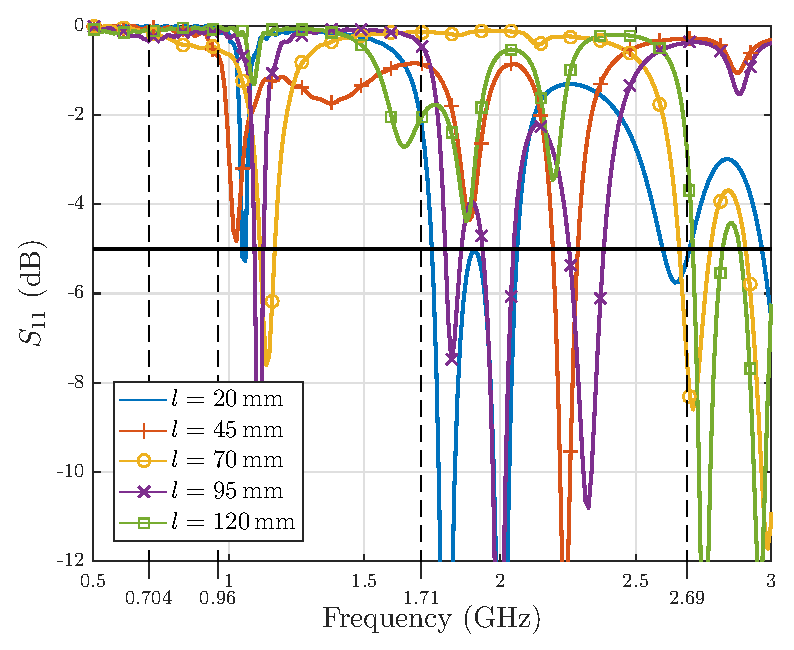
\includegraphics[width=\textwidth]{img/ant_length_long_res.eps}
        \caption{Antenna located on the side of the phone.}
        \label{fig:ant_length_long_res}
    \end{subfigure}
    \begin{subfigure}[b]{0.49\textwidth}
        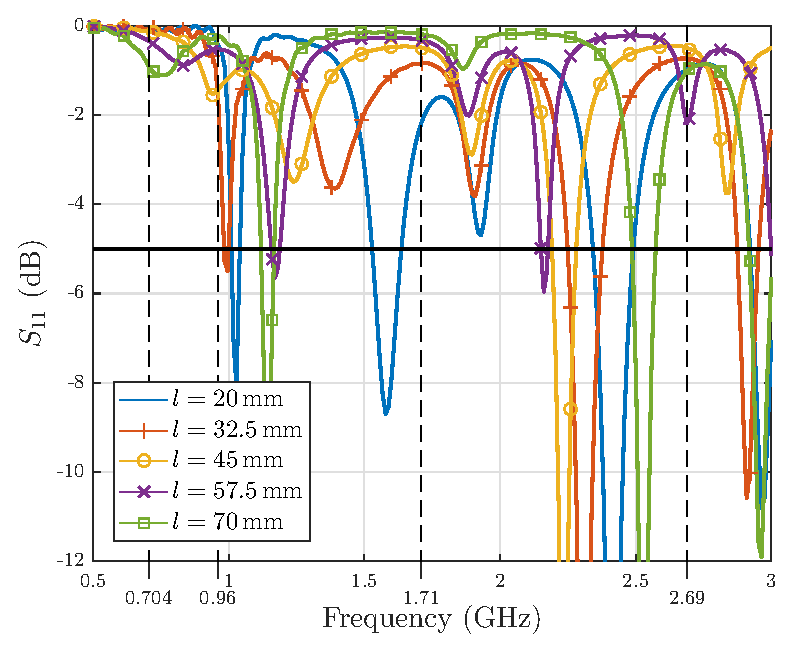
\includegraphics[width=\textwidth]{img/ant_length_short_res.eps}
        \caption{Antenna located on the top of the phone.}
        \label{fig:ant_length_short_res}
    \end{subfigure}
    \caption{The effect of antenna's length.}
    \label{fig:ant_length_result}
\end{figure}

The other matter affecting the size of an antenna besides length is its width. Impact of width is tested with the same structure that was used to test the effect of length, when the antenna is placed on the top of the phone. Antenna's length was also $70\,\milli\meter$ in this case. As Figure \ref{fig:width_res} presents, the effect of the width is quite minimal. Wider element gives a little bit better bandwidth in the both desired operational bands, but difference is not significant. Nevertheless the similarity of the results, larger bandwidth is more achievable with wider elements. Only it must be remembered, that the space for antennas is very limited on the sides of the phone, and thus, antennas cannot be much wider.

\begin{figure}[H]
    \centering
    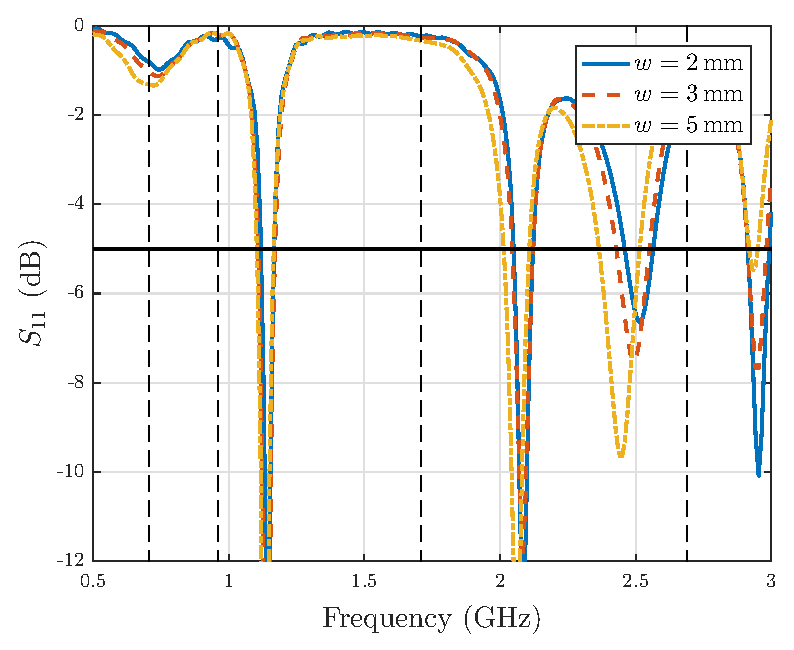
\includegraphics[width=0.5\textwidth]{img/width_res.eps}
    \caption{Effect of the width of an antenna.}
    \label{fig:width_res}
\end{figure}


\subsubsection{Location of the feed}
\label{sec:feed}
Besides the size of antenna, another interesting parameter is the location of the feed. This is tested with the same structure that was used to test the impact of the metallic back cover except for the small block on the corner, shown in Figure \ref{fig:metal_cover} earlier. Feeds are located in two ways: either on the long or the short side, like in Figures \ref{fig:ant_length_long} and \ref{fig:ant_length_short}, respectively. Feed is placed between the antenna and the ground plane, or the display in this case, and four different locations are tested on each side. The first position is in the corner of the ground plane, and the last is in the center of it. Between these are two positions at equal distances, denoted as ground 1/3 and ground 2/3.

Figures \ref{fig:feed_pos_side_res} and \ref{fig:feed_pos_top_res} show the simulation results for feed on the long side and feed on top, respectively. Both of these graphs yield the same conclusion: for the low band, feed provides better bandwidth when located at the corner of the ground plane. For the high band, feed location is the most promising when it is shifted away from the corner, and is located on the top side of the phone.

\begin{figure}[H]
    \centering
    \begin{subfigure}[b]{0.49\textwidth}
        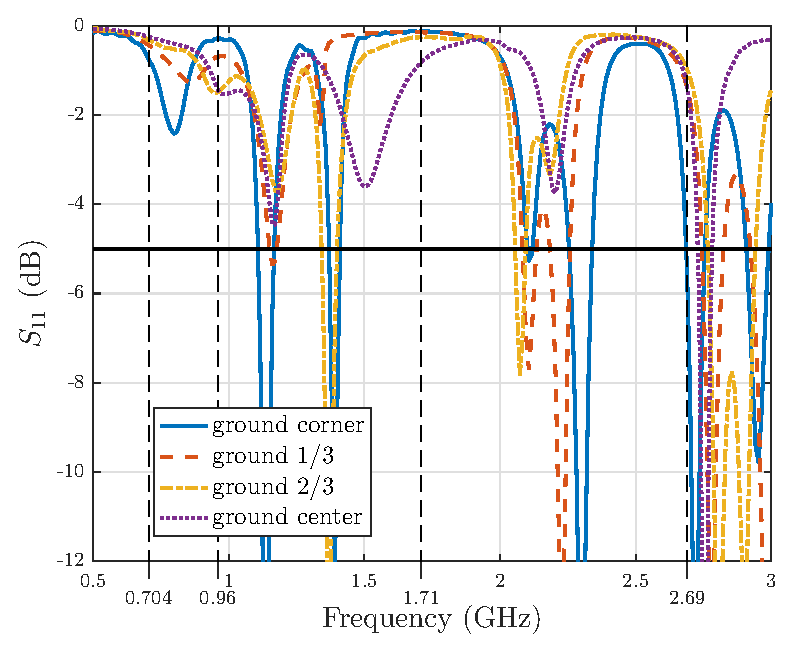
\includegraphics[width=\textwidth]{img/feed_pos_side_res.eps}
        \caption{Antenna located on the side of the phone.}
        \label{fig:feed_pos_side_res}
    \end{subfigure}
    \begin{subfigure}[b]{0.49\textwidth}
        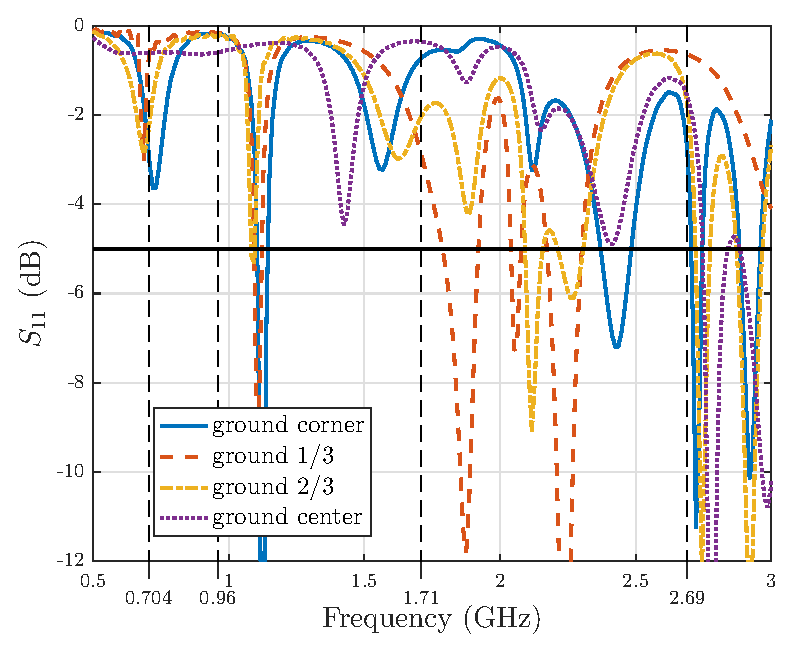
\includegraphics[width=\textwidth]{img/feed_pos_top_res.eps}
        \caption{Antenna located on the top of the phone.}
        \label{fig:feed_pos_top_res}
    \end{subfigure}
    \caption{The effect of the location of the feed.}
    \label{fig:feed_effect}
\end{figure}


\subsubsection{Position and shape of an antenna}
\label{sec:position_shape}

Positioning the antenna is as well worth testing. In this test, a $70\,\milli\meter$ long sheet is used, and it is bent over a corner to form an L-shaped structure. The total length of this element is the same as was one option in testing the effect of length, to have comparability. Antenna is positioned in one corner of the phone in four different ways presented in Table \ref{tab:l_structures}. The lengths on each side are kept the same, and positioning is changed by rotating the element. Feed is placed in the corner of the ground plane, and is oriented along either the long or the short side. Figure \ref{fig:l_shape_model} illustrates the model. In this illustration feed is placed on the long side of the phone.

Results are presented in Figure \ref{fig:l_shape_res}. The nature of each curve is very similar, especially other structures but 1, that are almost identical below ca. $2.3\,\giga\hertz$. As these three structures have quite strong resonance above $1\,\giga\hertz$, the blue curve of structure 1 is showing promising wideband performance. Although the good band is just above the low band, where performance of each setup is very weak, this test shows that wide band matching might be achievable with L-shaped elements in the corners.

\begin{table}[H]
    \centering
    \caption{Antenna parameters used while testing L-shaped antenna structures.}
    \label{tab:l_structures}
    \begin{tabular}{|M{0.22\textwidth}|M{0.22\textwidth}|M{0.22\textwidth}|M{0.22\textwidth}|}
        \hline
        \textbf{Antenna structure} & \textbf{Antenna length on the long side ($l_1$)} & \textbf{Antenna length on the short side ($l_2$)} & \textbf{Feed orientation}\\
        \hline
         Structure A & $50\,\milli\meter$ & $20\,\milli\meter$ & On the long side\\
         \hline
         Structure B & $50\,\milli\meter$ & $20\,\milli\meter$ & On the short side\\
         \hline   
         Structure C & $20\,\milli\meter$ & $50\,\milli\meter$ & On the short side\\
         \hline
         Structure D & $20\,\milli\meter$ & $50\,\milli\meter$ & On the long side\\
         \hline
    \end{tabular}
\end{table}

\begin{figure}[H]
    \centering
    \begin{subfigure}[b]{0.49\textwidth}
        \includegraphics[width=\textwidth]{img/L_shape.eps}
        \caption{Model of L-shaped antenna.}
        \label{fig:l_shape_model}
    \end{subfigure}
    \begin{subfigure}[b]{0.49\textwidth}
        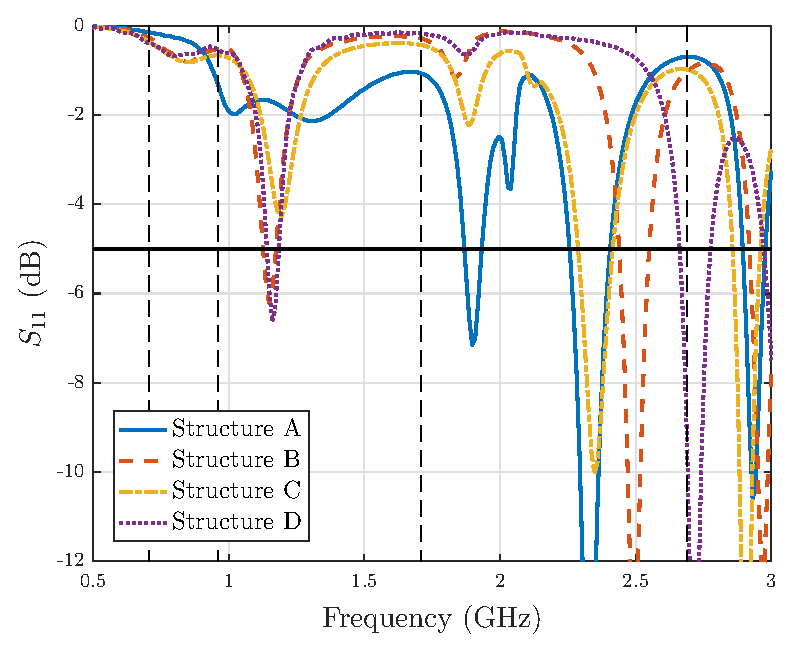
\includegraphics[width=\textwidth]{img/L_shape_res.eps}
        \caption{Results from simulations.}
        \label{fig:l_shape_res}
    \end{subfigure}
    \caption{Simulated L-shaped antennas.}
    \label{fig:l_shape}
\end{figure}

So far all investigated antennas have been either straight, rectangular sheets or L-shaped elements. Modifying the shape more might enable to excite different resonant modes. Figure \ref{fig:shape_models} shows six shapes of different complexity implemented on the top of the handset. All the tested structures are fed from the same corner of the ground plane. To make it clear, the antennas of shapes 4, 5, and 6 (\Cref{fig:shape4,fig:shape5,fig:shape6}, respectively) are $0.5\,\milli\meter$ apart from the cover.

\begin{figure}[H]
    \centering
    \begin{subfigure}[b]{0.3\textwidth}
        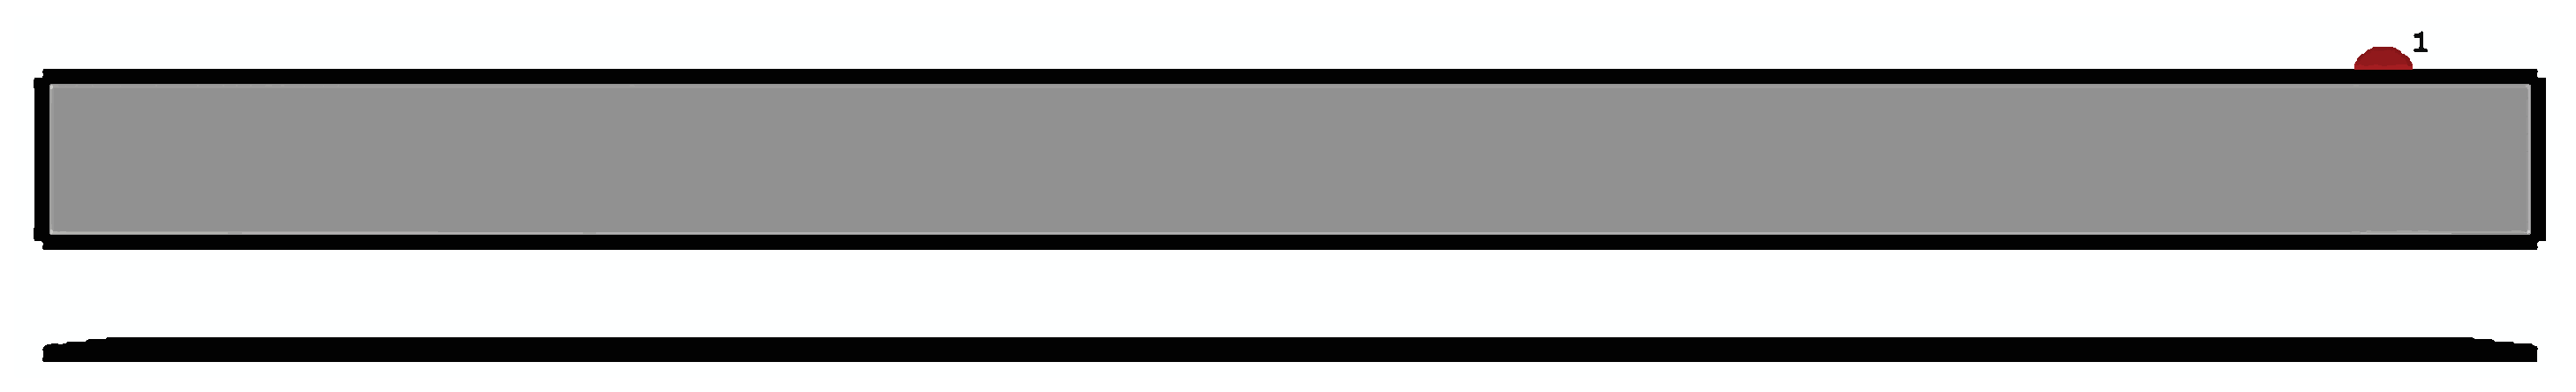
\includegraphics[width=\textwidth]{img/shape1.eps}
        \caption{Shape 1.}
        \label{fig:shape1}
    \end{subfigure}
    \begin{subfigure}[b]{0.3\textwidth}
        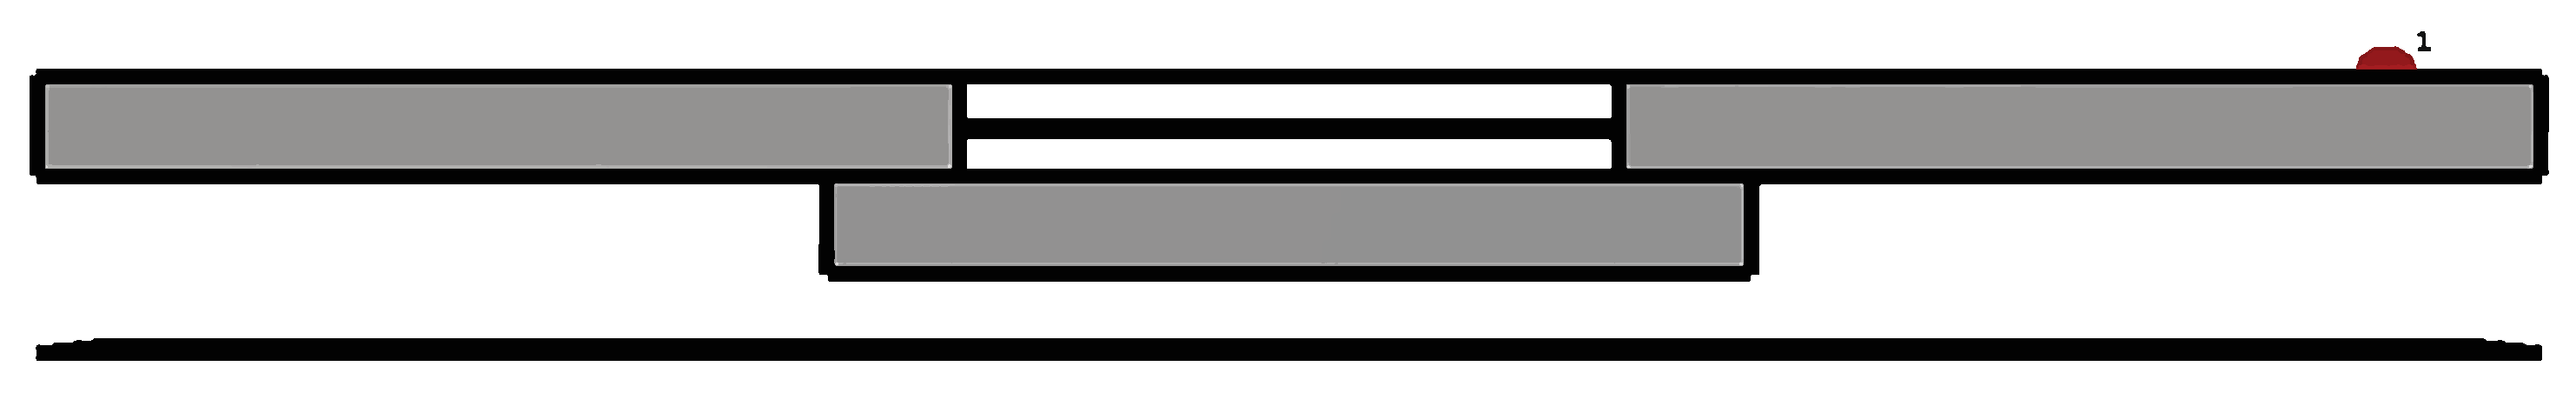
\includegraphics[width=\textwidth]{img/shape2.eps}
        \caption{Shape 2.}
        \label{fig:shape2}
    \end{subfigure}
    \begin{subfigure}[b]{0.3\textwidth}
        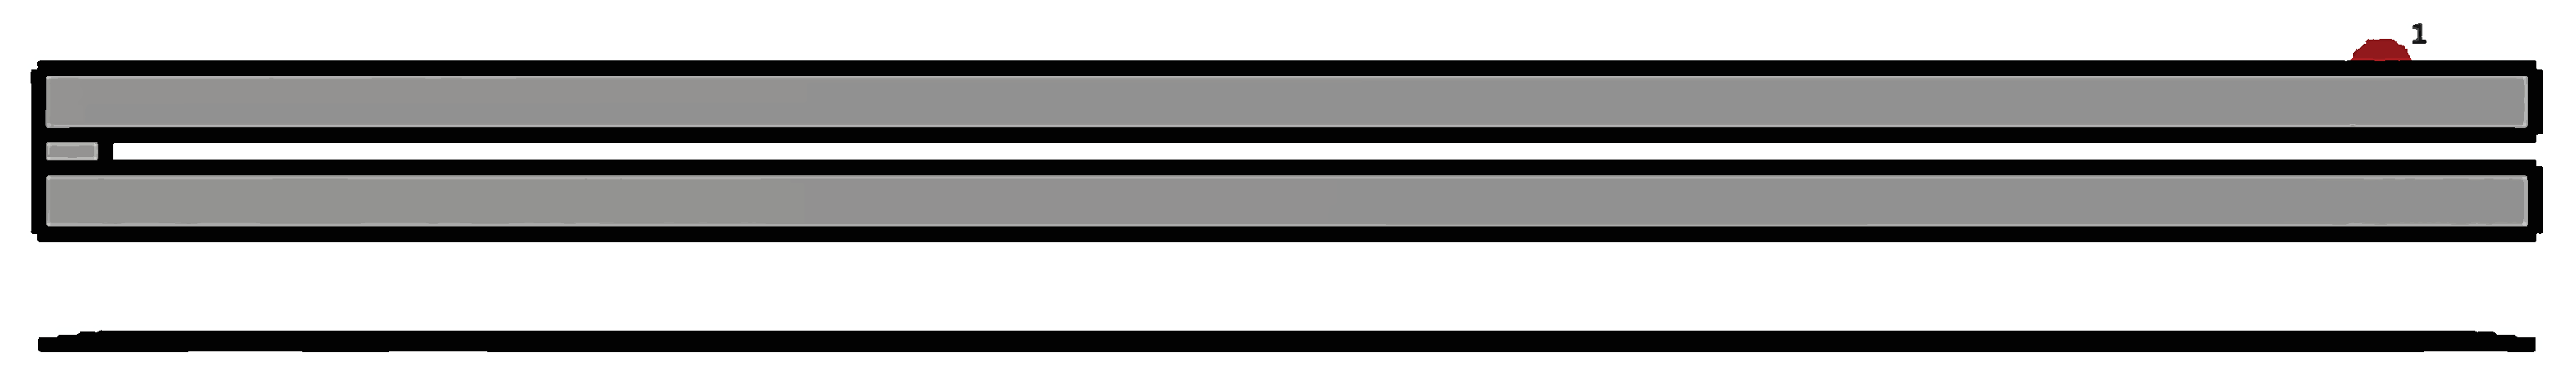
\includegraphics[width=\textwidth]{img/shape3.eps}
        \caption{Shape 3.}
        \label{fig:shape3}
    \end{subfigure}
    
    \begin{subfigure}[b]{0.3\textwidth}
        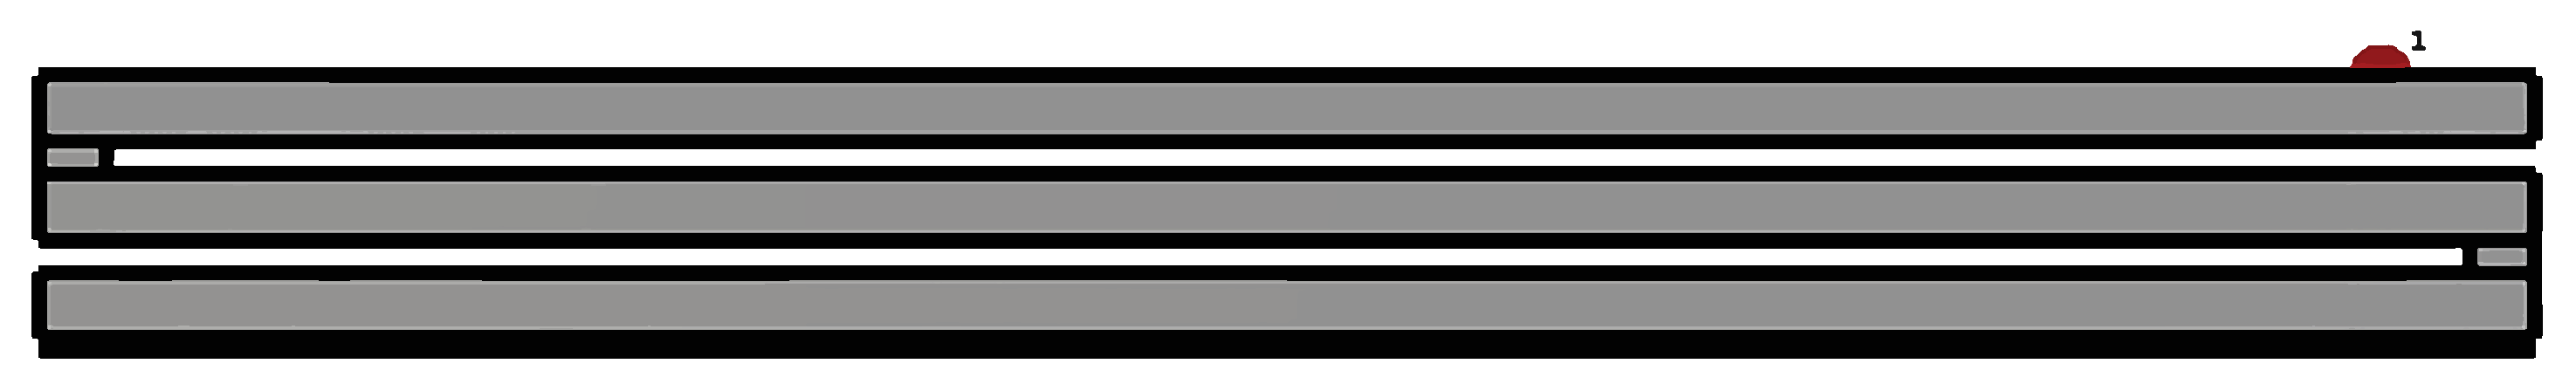
\includegraphics[width=\textwidth]{img/shape4.eps}
        \caption{Shape 4.}
        \label{fig:shape4}
    \end{subfigure}
    \begin{subfigure}[b]{0.3\textwidth}
        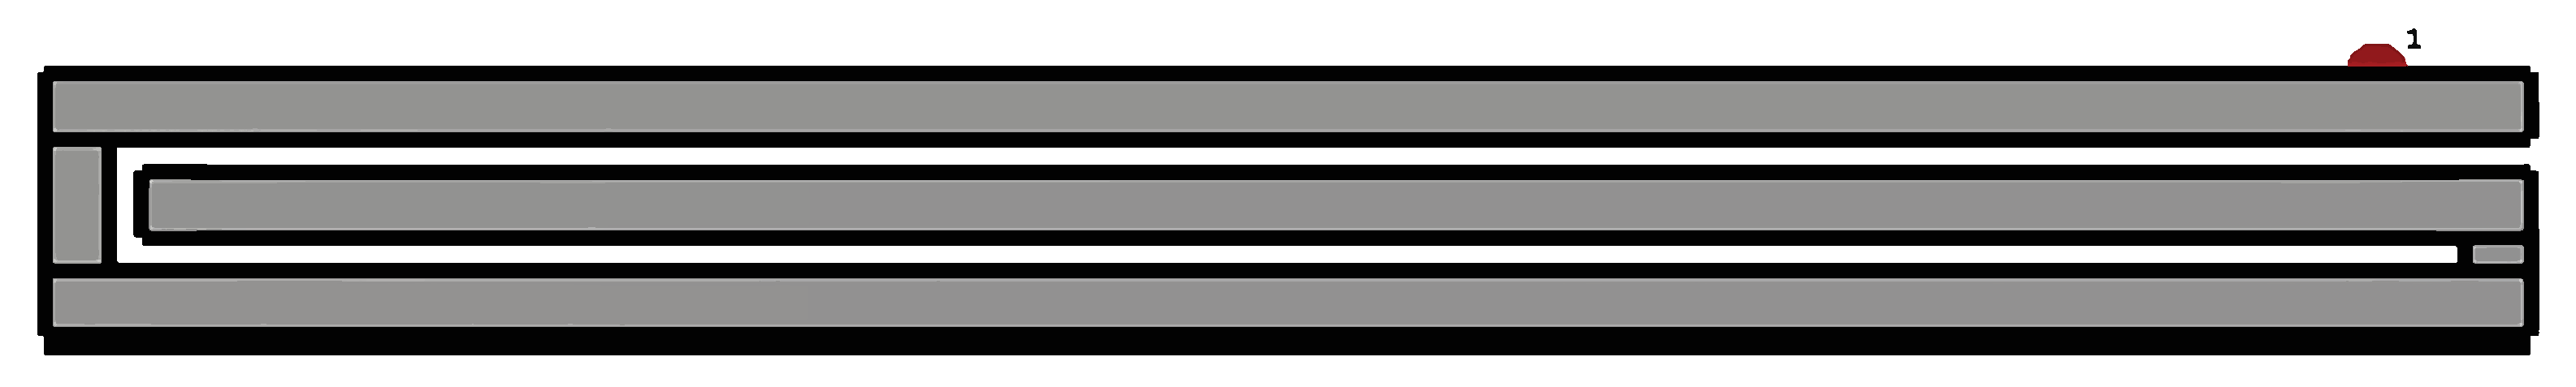
\includegraphics[width=\textwidth]{img/shape5.eps}
        \caption{Shape 5.}
        \label{fig:shape5}
    \end{subfigure}
    \begin{subfigure}[b]{0.3\textwidth}
        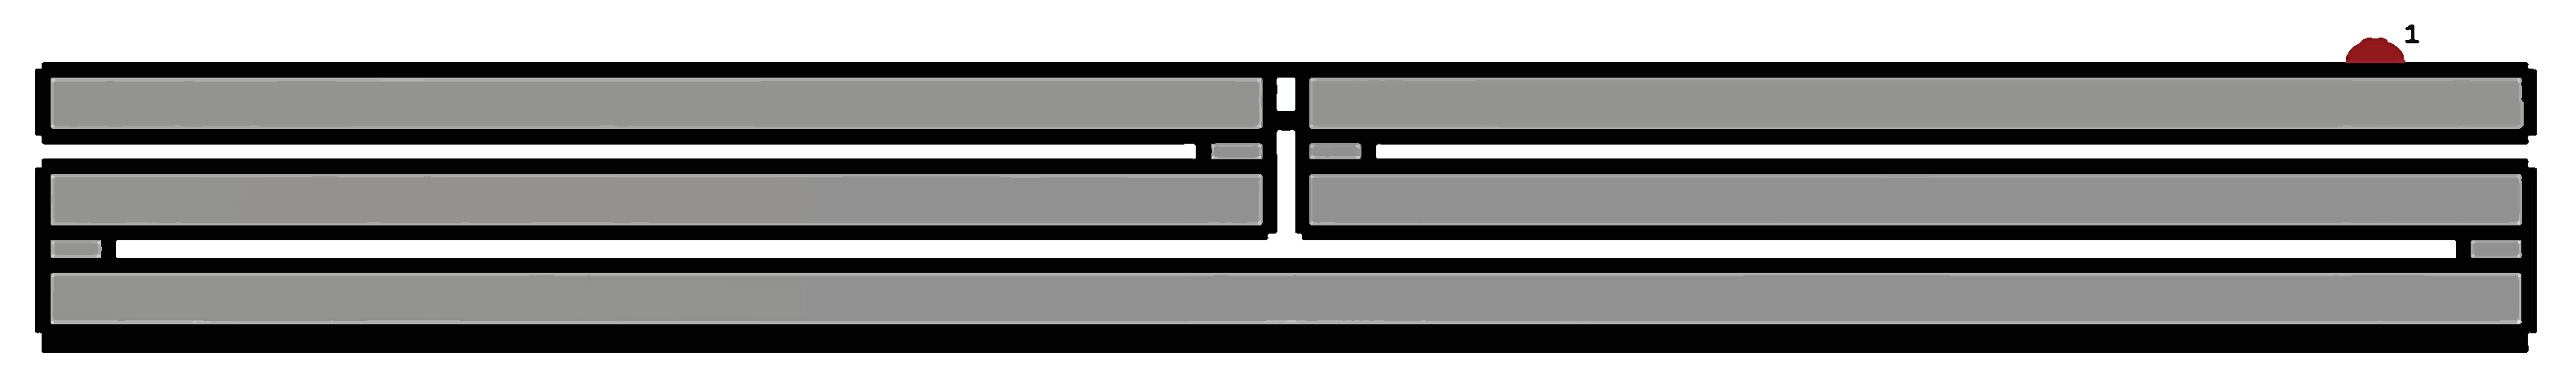
\includegraphics[width=\textwidth]{img/shape6.eps}
        \caption{Shape 6.}
        \label{fig:shape6}
    \end{subfigure}
    \caption{Different shapes for antenna located at the end of the phone.}
    \label{fig:shape_models}
\end{figure}

Results can be seen in Figure \ref{fig:shape}. For the low band, shape 4 has the best matching and quite good bandwidth. The two most simple shapes, 1 and 2, produce almost identical results, and in the lowest frequencies they are somewhat wideband, though the matching level is poor. These simpler structures also operate better in the high band than other tested antennas.

\begin{figure}[H]
    \centering
    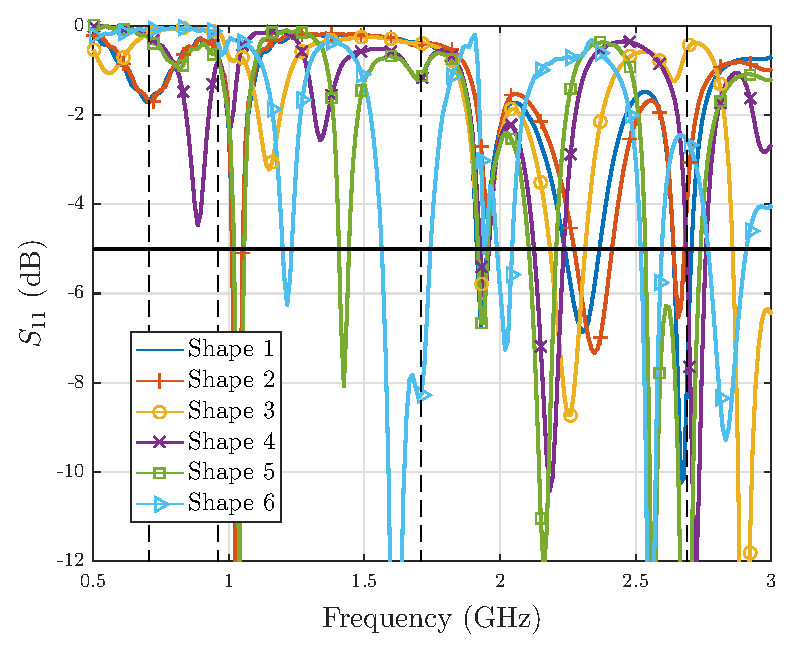
\includegraphics[width=0.5\textwidth]{img/shape.eps}
    \caption{Effect of different antenna shapes. Antennas are located at the end of a phone.}
    \label{fig:shape}
\end{figure}

As was shown in earlier Figure \ref{fig:metal_rim}, possible locations for antennas are above and below the display of the phone. Therefore, an antenna element is placed in that area, illustrated in Figure \ref{fig:front_model}, and compared to a similar element located on the top of the phone, like shown in Figure \ref{fig:shape1}. It can be seen from Figure \ref{fig:front_res} that the difference between these two locations is minimal. The shapes of the responses are nearly identical in the low frequencies, and they follow the same pattern in the higher band. Matching levels at the low band are bad, but the bandwidth is quite wide. In the high band, the element on the front gives good matching on two sub-bands, and is promising in the rest of the band also.

\begin{figure}[H]
    \centering
    \begin{subfigure}[b]{0.49\textwidth}
        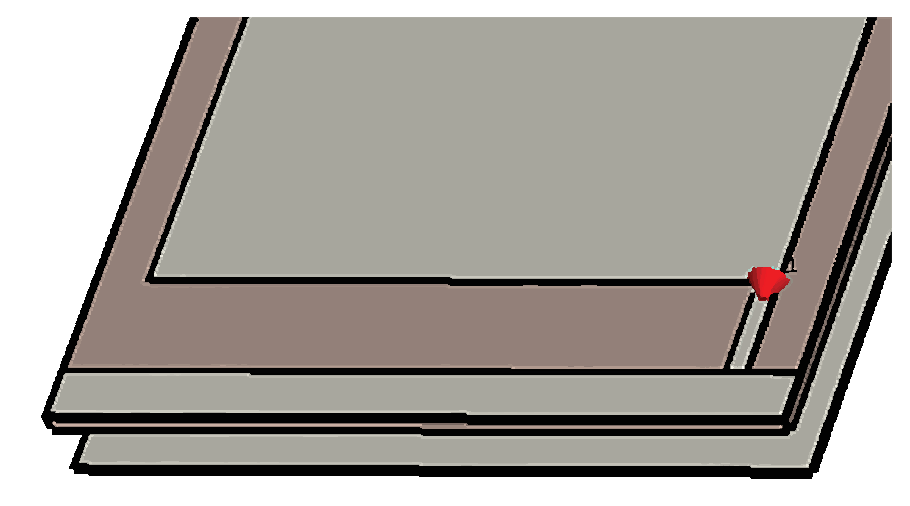
\includegraphics[width=\textwidth]{img/front.eps}
        \caption{Model of frontside antenna element.}
        \label{fig:front_model}
    \end{subfigure}
    \begin{subfigure}[b]{0.49\textwidth}
        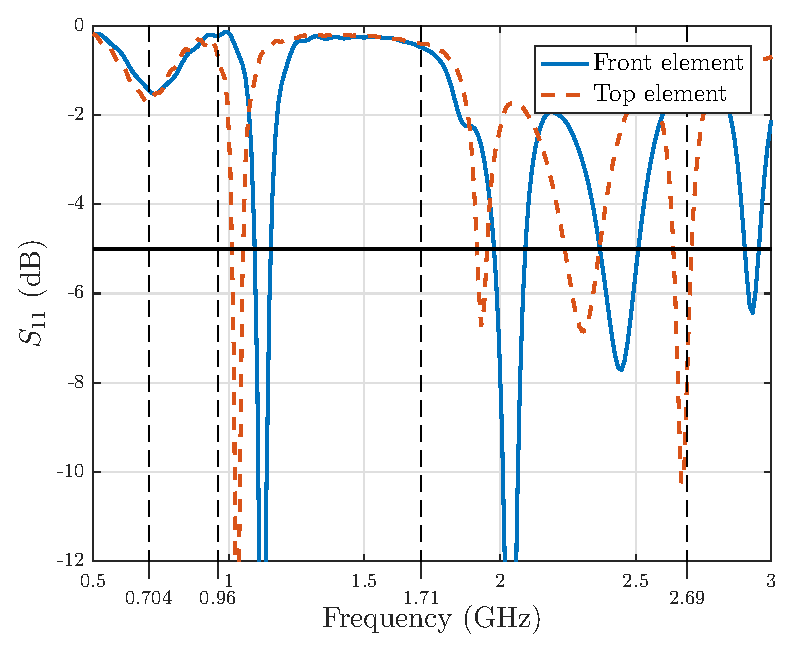
\includegraphics[width=\textwidth]{img/front_res.eps}
        \caption{Results from simulations.}
        \label{fig:front_res}
    \end{subfigure}
    \caption{Antenna element on the front side of the phone.}
    \label{fig:front_elem}
\end{figure}



In addition to straight sheets, slots can be added to elements to introduce new wave modes. This test has the same antenna as presented in Figure \ref{fig:metal_cover}, with one or two slots on the sides. The first slot on the long side, at $20\,\milli\meter$ from the end, and second is on the short side at the same distance from the end of the element. Both slots are $2\,\milli\meter$ wide.

Adding one slot creates strong and very narrow peak at low band, as can be seen from Figure \ref{fig:slot_res}. Second slot gives slightly wider bandwidth, but decreases matching level compared to zero or one slot.

\begin{figure}[H]
    \centering
    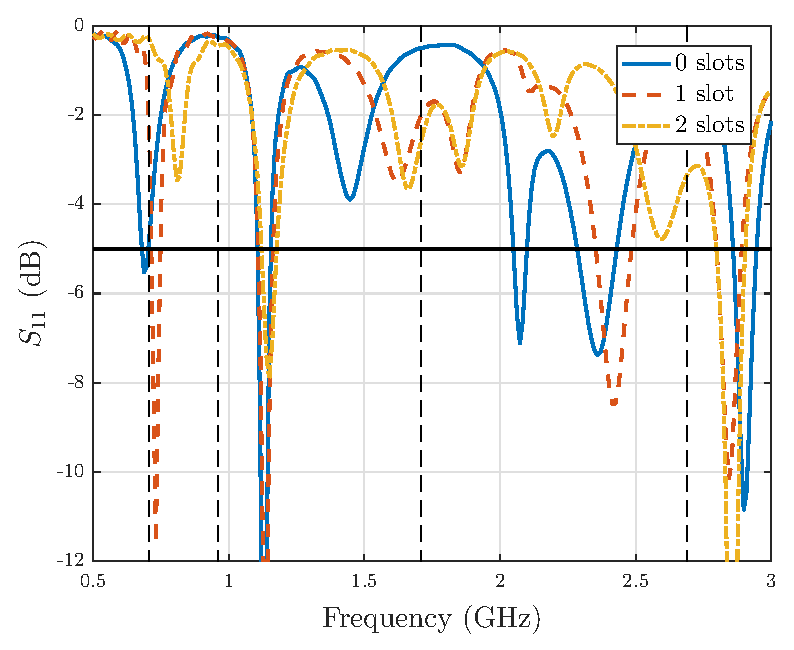
\includegraphics[width=0.5\textwidth]{img/slot_res.eps}
    \caption{Effect of slots in the antenna element.}
    \label{fig:slot_res}
\end{figure}

\subsubsection{Ground plane}
\label{sec:ground_plane}
Last thing to investigate is the effect of ground plane. So far phone's display has been used as a ground plane, but since the back cover is also large metallic plate, that could be used as well as a ground. The test setup is the same as was used to the effect of metal cover, shown in Figure \ref{fig:metal_cover}. Only feed is moved between the iterations. Figure \ref{fig:ground_plane} shows the impact. When feed is moved to locate between the back cover and antenna element, the response is much smoother, and has wider bandwidths and better matching levels. One possible explanation for this behavior might rely on the sizes of the two planes. When display is used as a ground plane, the larger back cover interacts with the EM-fields stronger and therefore is more harmful for the antennas. If feed is grounded to the back cover, then the disturbing element is smaller and negative effects are not as strong.

\begin{figure}[H]
    \centering
    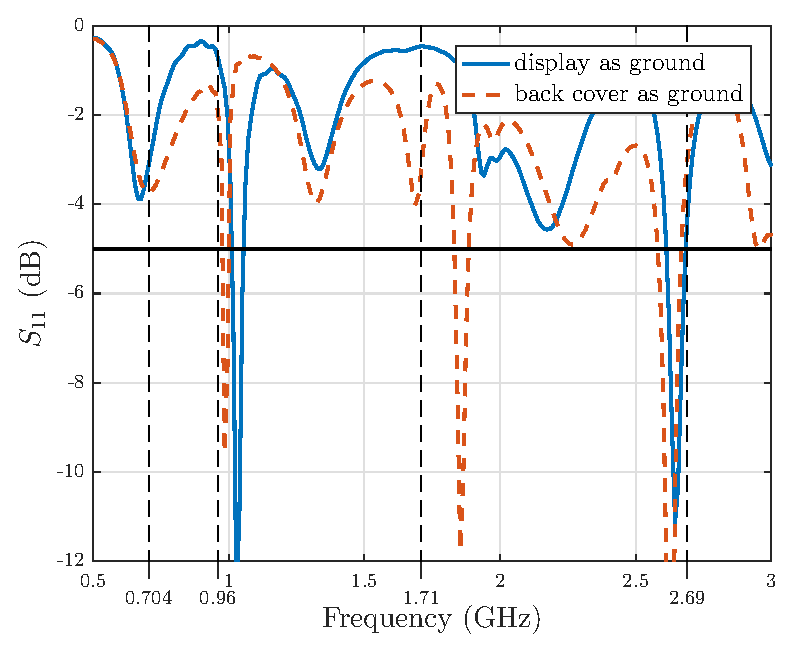
\includegraphics[width=0.5\textwidth]{img/ground_vs_display.eps}
    \caption{Effect of using display or back cover as ground plane.}
    \label{fig:ground_plane}
\end{figure}

\subsubsection{Summary of the pre-study}
\label{sec:pre_study_summary}
The conclusions made from all these presented simulation results are collected and summarized in Table \ref{tab:dimension_summary} below. 

\begin{table}[H]
    \centering
    \caption{Summary of how changing dimensions affect antenna's performance.}
    \label{tab:dimension_summary}
    \begin{tabular}{|p{0.28\textwidth}|p{0.65\textwidth}|}
        \hline
        \textbf{Changed parameter} & \textbf{Impact on antenna's performance} \\
        \hline
        Element length on the side of the phone & Resonance frequencies variate and longer elements tend to lower the frequency.\\
        \hline
        Element length on the end of the phone & Resonance frequencies variate and longer elements tend to lower the frequency.\\
        \hline
        Element on the front side of the phone & Adding element improves matching levels.\\
        \hline
        Element width & Wider element slightly increases bandwidth.\\
        \hline
        Location of the feed & Feed close to a corner of the display gives wider band, although resonance is smoother if feed is in the center.\\
        \hline
        Ground plane & Using back cover as a ground plane instead of the display gives wider bandwidths and more resonating frequencies.\\
        \hline
        Shape of the element & The more complex the element is, the more it resonates. Large loops increase bandwidth. Elements bended over the corner (L-shaped) even resonances and improve matching levels.\\
        \hline
        Slots & Slots in the element on the long side narrow bands and on the short side decrease matching levels.\\
        \hline
    \end{tabular}
\end{table} 

\clearpage